\chapter{Experimentaciones y Resultados}\label{chapter:results}

En la presente sección comenzamos mostrando los sistemas de cómputo utilizados para la experimentación.
Seguidamente, dividimos este capítulo en seis secciones.
Primero, se muestra los resultados de la optimización del \emph{bend}.
Para ello se inicia mostrando en tres gráficas distintas el desempeño de cada algoritmo en 
las tres etapas de la estrategia de optimización; luego, se detalla los resultados por cada algoritmo
de manera individual.
Segundo, se realiza un análisis al diseño del \emph{bend} mejor optimizado.
Tercero, de manera similar al caso del \emph{bend}, se expone los resultado de la optimización del WDM.
Cuarto, se desarrolla un análisis al diseño del WDM mejor optimizado.
Quinto, se realiza una discusión crítica sobre los resultados de la optimización del \emph{bend}.
Finalmente, se realiza una discusión similar sobre los resultados del WDM.

Los experimentos se realizaron en tres equipos brindados por la Universidad de Ingeniería y Tecnología:

\begin{enumerate}
  \item Un Intel Core i7-3770K 3.50 GHz con 8 cores y 32 GB de RAM.
        Este computador contó con un GPU NVIDIA Quadro RTX 4000 con 8GB GDDR6.

  \item Del \emph{cluster} Khipu, un Intel Xeon Gold 6230 2.10 GHz con 40 \emph{cores} y 128 GB de RAM.
        Este nodo contó con un GPU NVIDIA Tesla T4 con 16 GB GDDR6.

  \item Del \emph{cluster} Khipu, un AMD EPYC 7742 2.25 GHz con 128 \emph{cores} y 1024 GB de RAM.
        Este nodo contó con un GPU NVIDIA Ampere A100 con 40 GB HMB2.

\end{enumerate}

Sacando la media geométrica de los tiempos calculados, el tiempo promedio de simulación en los tres 
sistemas en cada etapa de la estrategia de optimización se detalla en la \autoref{tab:times} (el signo -
indica que en ese sistema de cómputo no se realizaron experimentos con ese dispositivo).

\begin{table}[ht]
    \centering
    \begin{tabular}{|c|c|c|c|}
    \hline 
      Tiempo promedio (s) &  Quadro RTX & Tesla T4 & Ampere A100 \\
    \hline 
      Optimización continua (\emph{bend})            & 14.261 & 15.432 & - \\
      Optimización discreta (\emph{bend})            & 15.961 & 18.718 & - \\
      Optimización de fabricación (\emph{bend})      & 47.084 & 50.639 & - \\
      Optimización continua (WDM)                    & 16.876 & - & 17.479 \\
      Optimización discreta (WDM)                    & 18.431 & - & 19.780 \\
      Optimización de fabricación (WDM)              & 53.941 & - & 55.406 \\
    \hline 
    \end{tabular}
    \caption{Tiempos promedio de simulación en cada etapa de optimización para el \emph{bend} y WDM con los
    tres sistemas de cómputo usados.}
    \label{tab:times}
\end{table}

Por cada optimización se realizó como máximo $2000$ evaluaciones de $f_{obj}$ en la optimización continua,
$3 \times 800$ en la optimización discreta y $3 \times 400$ en la optimización de fabricación.
Así, por ejemplo, usando Quadro RTX la optimización de un \emph{bend} podía tomar hasta 34 horas
y usando Ampere A100 la optimización de un WDM podía tomar hasta 41 horas.
Es importante destacar que con estas estimaciones se está obviando factores como
el tiempo de escritura en disco para los \emph{logs} y 
el tiempo de ejecución de cada algoritmo, simplemente se está considerando
el tiempo desde que se envía una solicitud a Maxwell-B para simular un dispositivo en el GPU
hasta el momento que SPINS-B recibe el resultado.

Por otro lado, cada GPU solo puede realizar una simulación a la vez, en caso de querer 
evaluar dos parametrizaciones al mismo tiempo una era puesta en cola. De este modo,
siendo el tiempo de simulación el cuello de botella de las optimizaciones, los programas simplemente
se ejecutaron con un solo \emph{core} y se limitó la memoria a 32 GB para los nodos del \emph{cluster}
Khipu mediante SLURM (herramienta que funciona como gestor de recursos de Khipu).


En las siguientes secciones las imágenes que muestran resultados de simulación del \emph{bend} o WDM
incluyen un círculo blanco, este representa una circunferencia de radio $r_f = 80 nm$,
el mínimo radio de curvatura que se está intentando imponer.
Además, las imágenes que resumen el proceso de optimización de cada dispositivo incluyen
rectas horizontales punteadas por un tema de visualización (distintos algoritmos-iteraciones
alcanzaron condiciones para detenerse antes de alcanzar la máxima cantidad permitida de
evaluaciones del FOM), estas rectas simplemente extienden el mejor resultado obtenido.

\section{Resultados de Optimización del \emph{Bend}}\label{sec:results-bend}

En la \autoref{fig:bend-cont}, \autoref{fig:bend-disc} y \autoref{fig:bend-fab} se observa 
el desempeño de los cinco algoritmos seleccionados en la etapa de optimización continua, discreta y
de fabricación del \emph{bend}, respectivamente.
Los resultados en más detalle por algoritmo se pueden encontrar en la 
\autoref{tab:opt-LBFGSB-bend} (L-BFGS-B),
\autoref{tab:opt-CMA-bend} (G-CMA-ES),
\autoref{tab:opt-MMA-bend} (MMA),
\autoref{tab:opt-PSO-bend} (G-PSO) y
\autoref{tab:opt-GA-bend} (G-GA).

\begin{landscape}
\begin{figure}[ht]
  \centering
  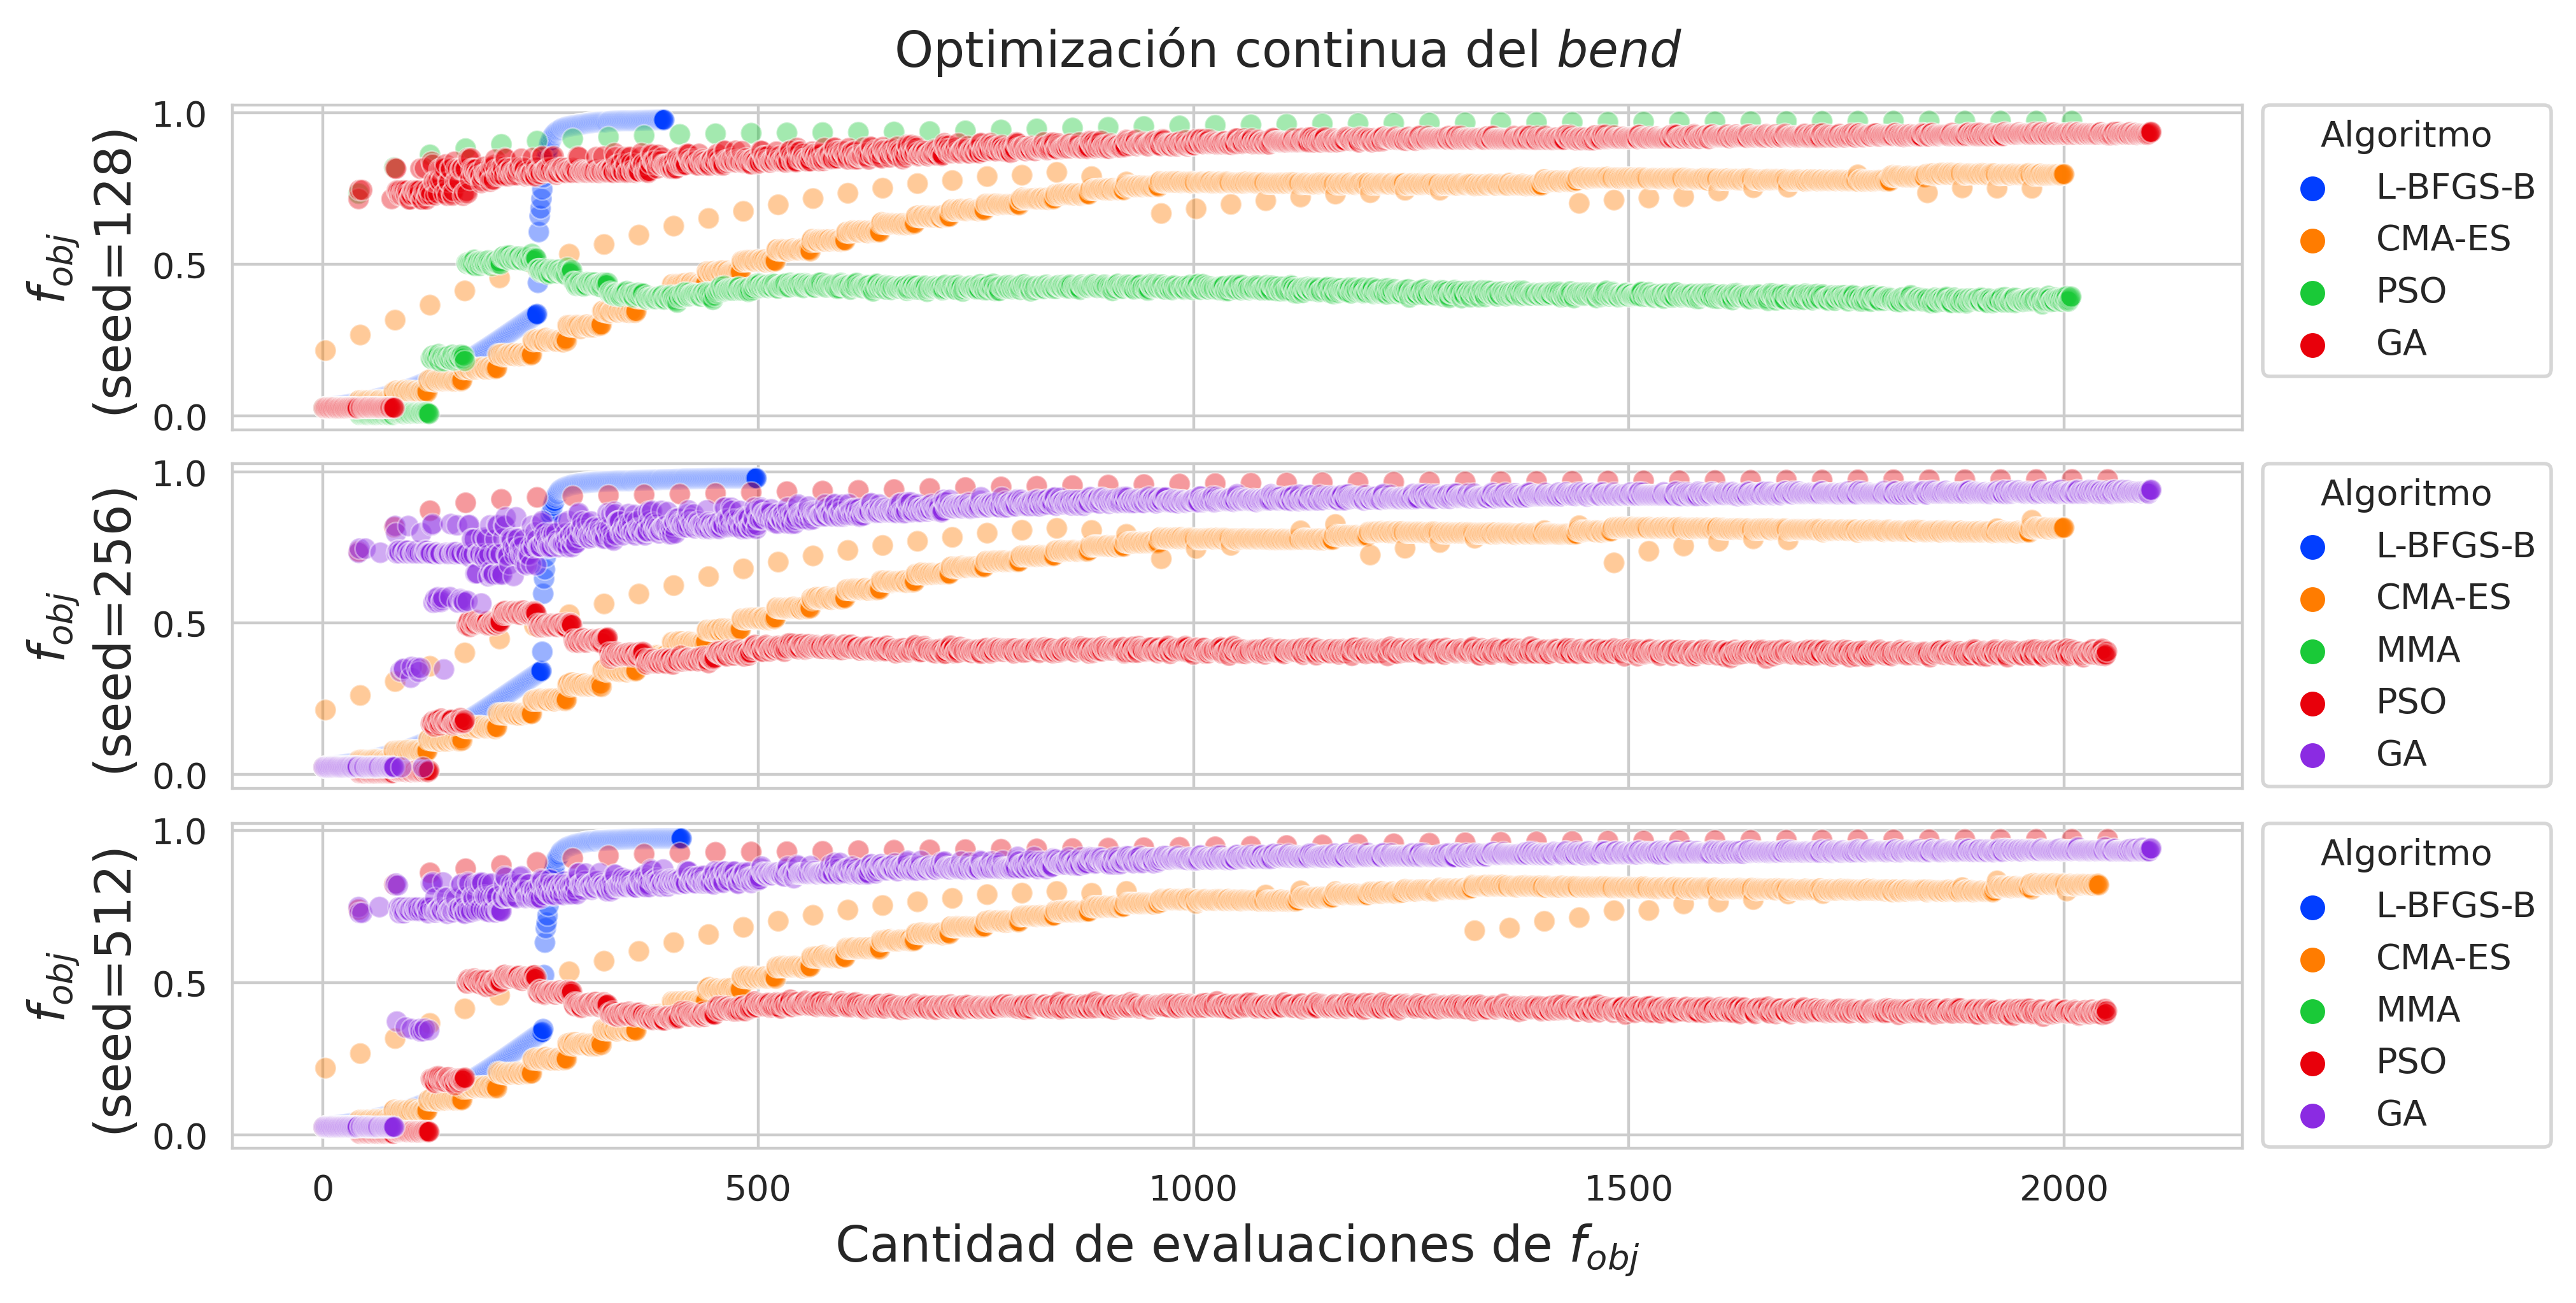
\includegraphics[scale=1.0]{image/results/bend/bend-opt-cont.png}
  \caption{Gráfico de valores de $f_{obj}$ obtenidos por los algoritmos en la optimización continua del \emph{bend}}
  \label{fig:bend-cont}
\end{figure}
\end{landscape}

\begin{landscape}
\begin{figure}[ht]
  \centering
  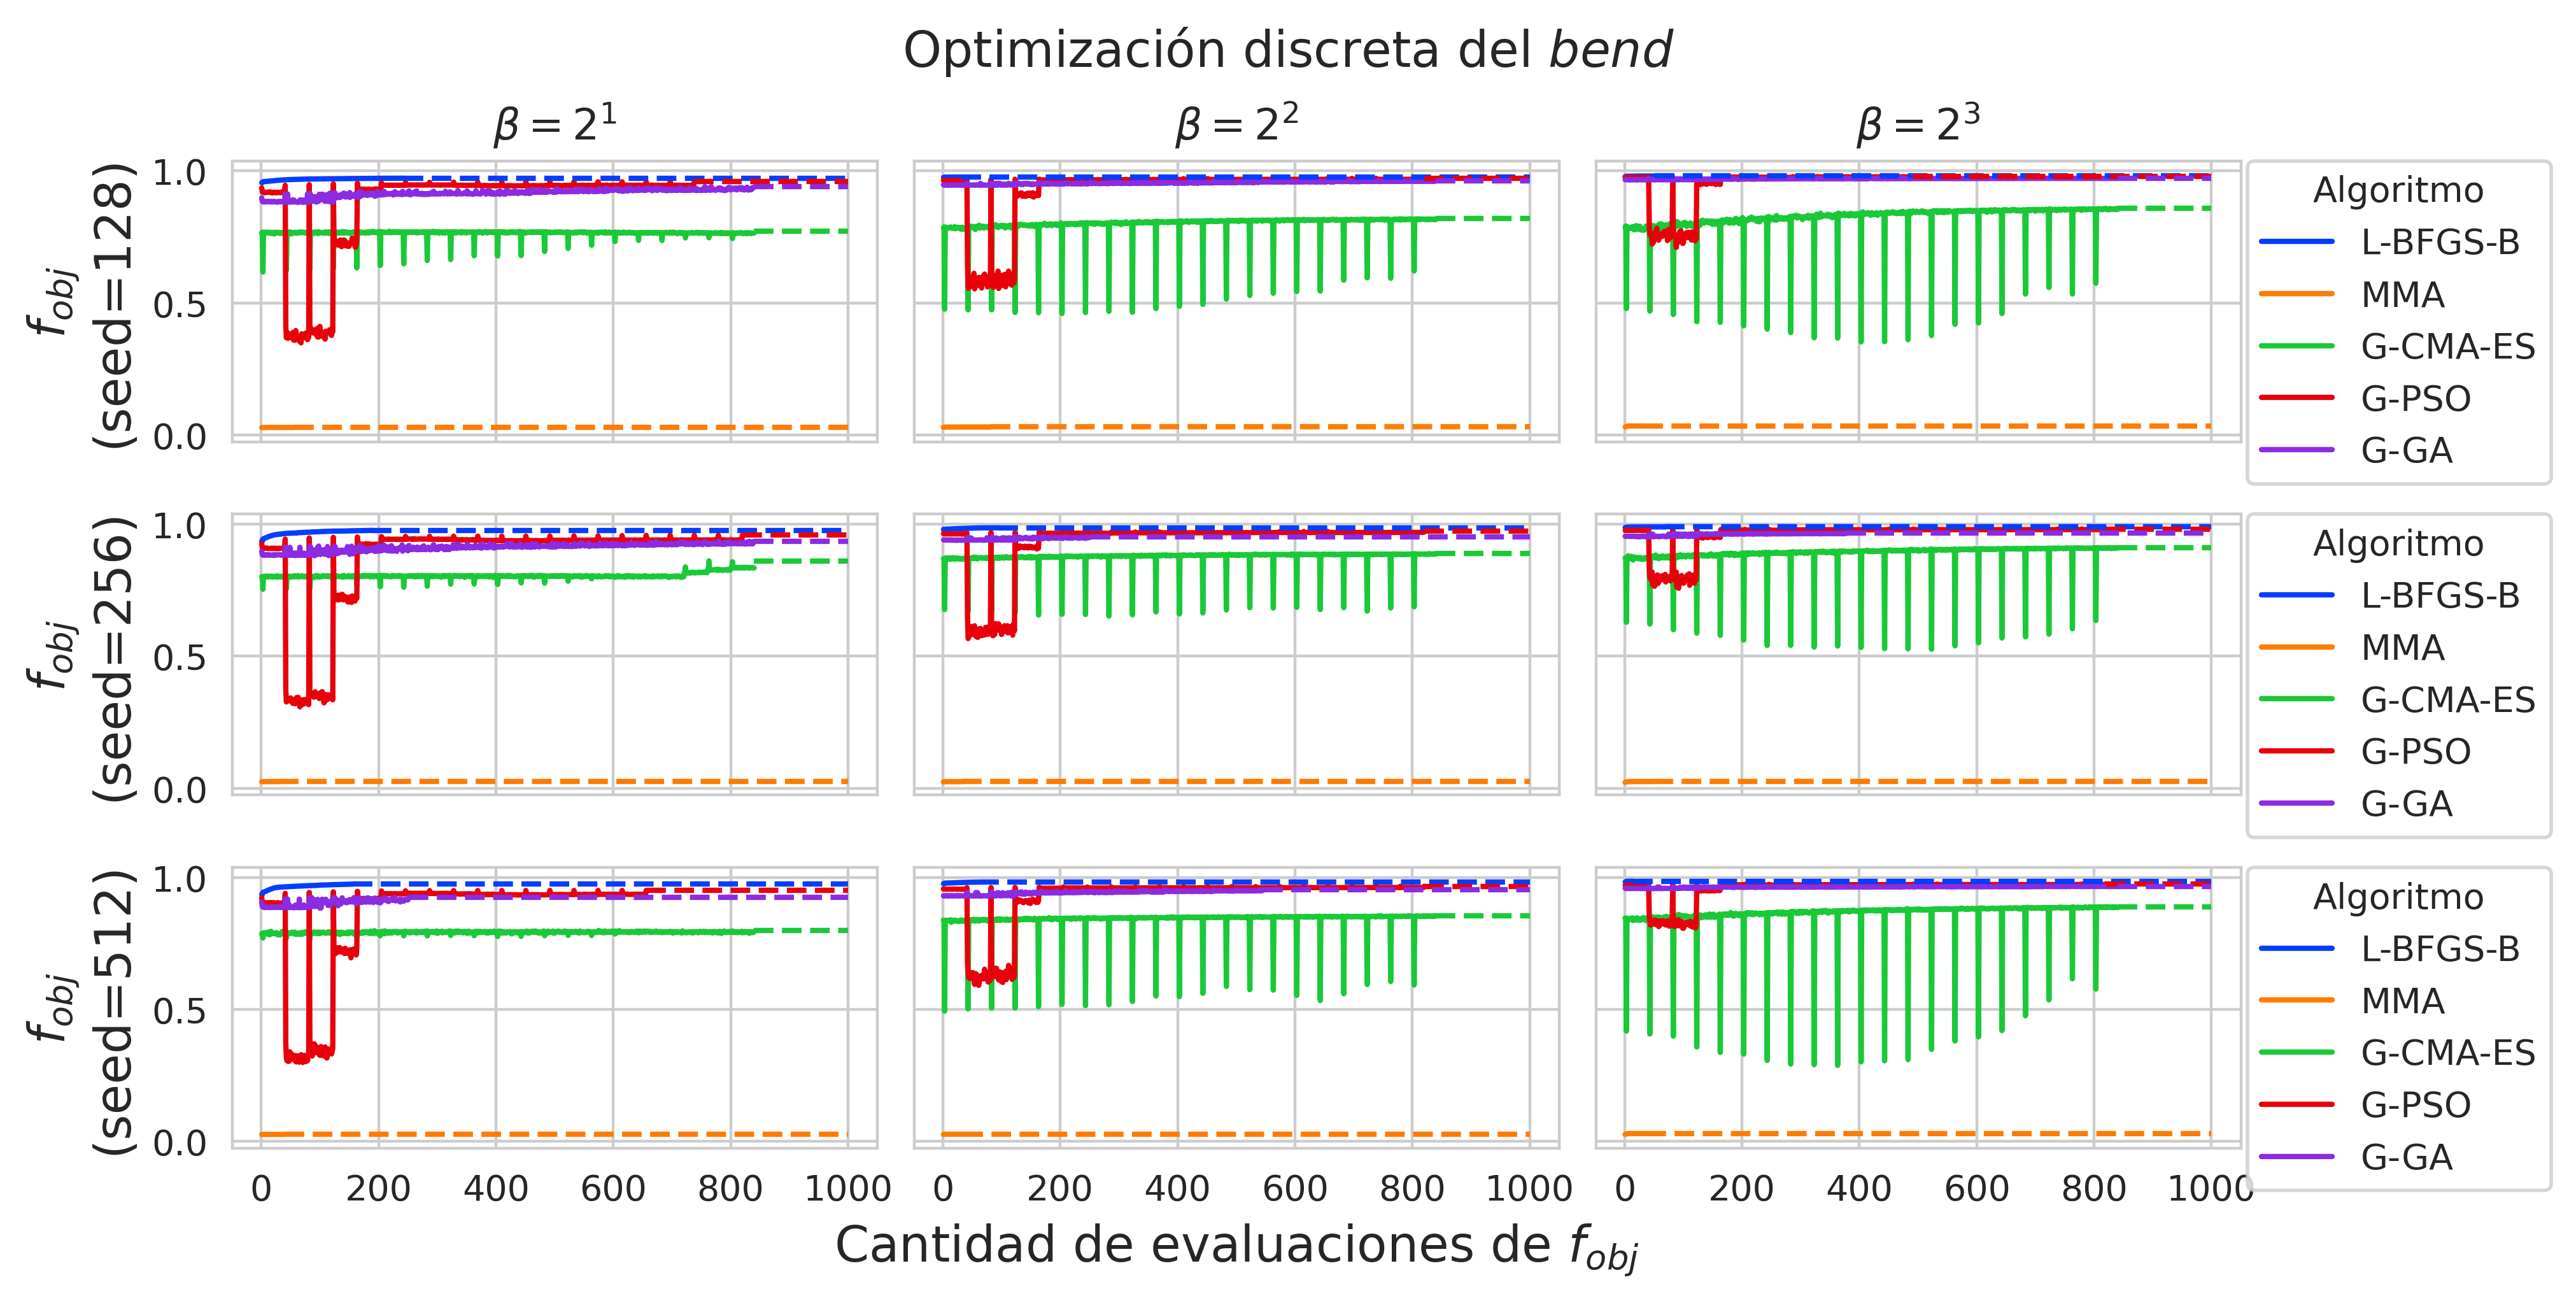
\includegraphics[scale=1.0]{image/results/bend/bend-opt-disc.png}
  \caption{Gráfico de valores de $f_{obj}$ obtenidos por los algoritmos en la optimización discreta del \emph{bend}}
  \label{fig:bend-disc}
\end{figure}
\end{landscape}

\begin{landscape}
\begin{figure}[ht]
  \centering
  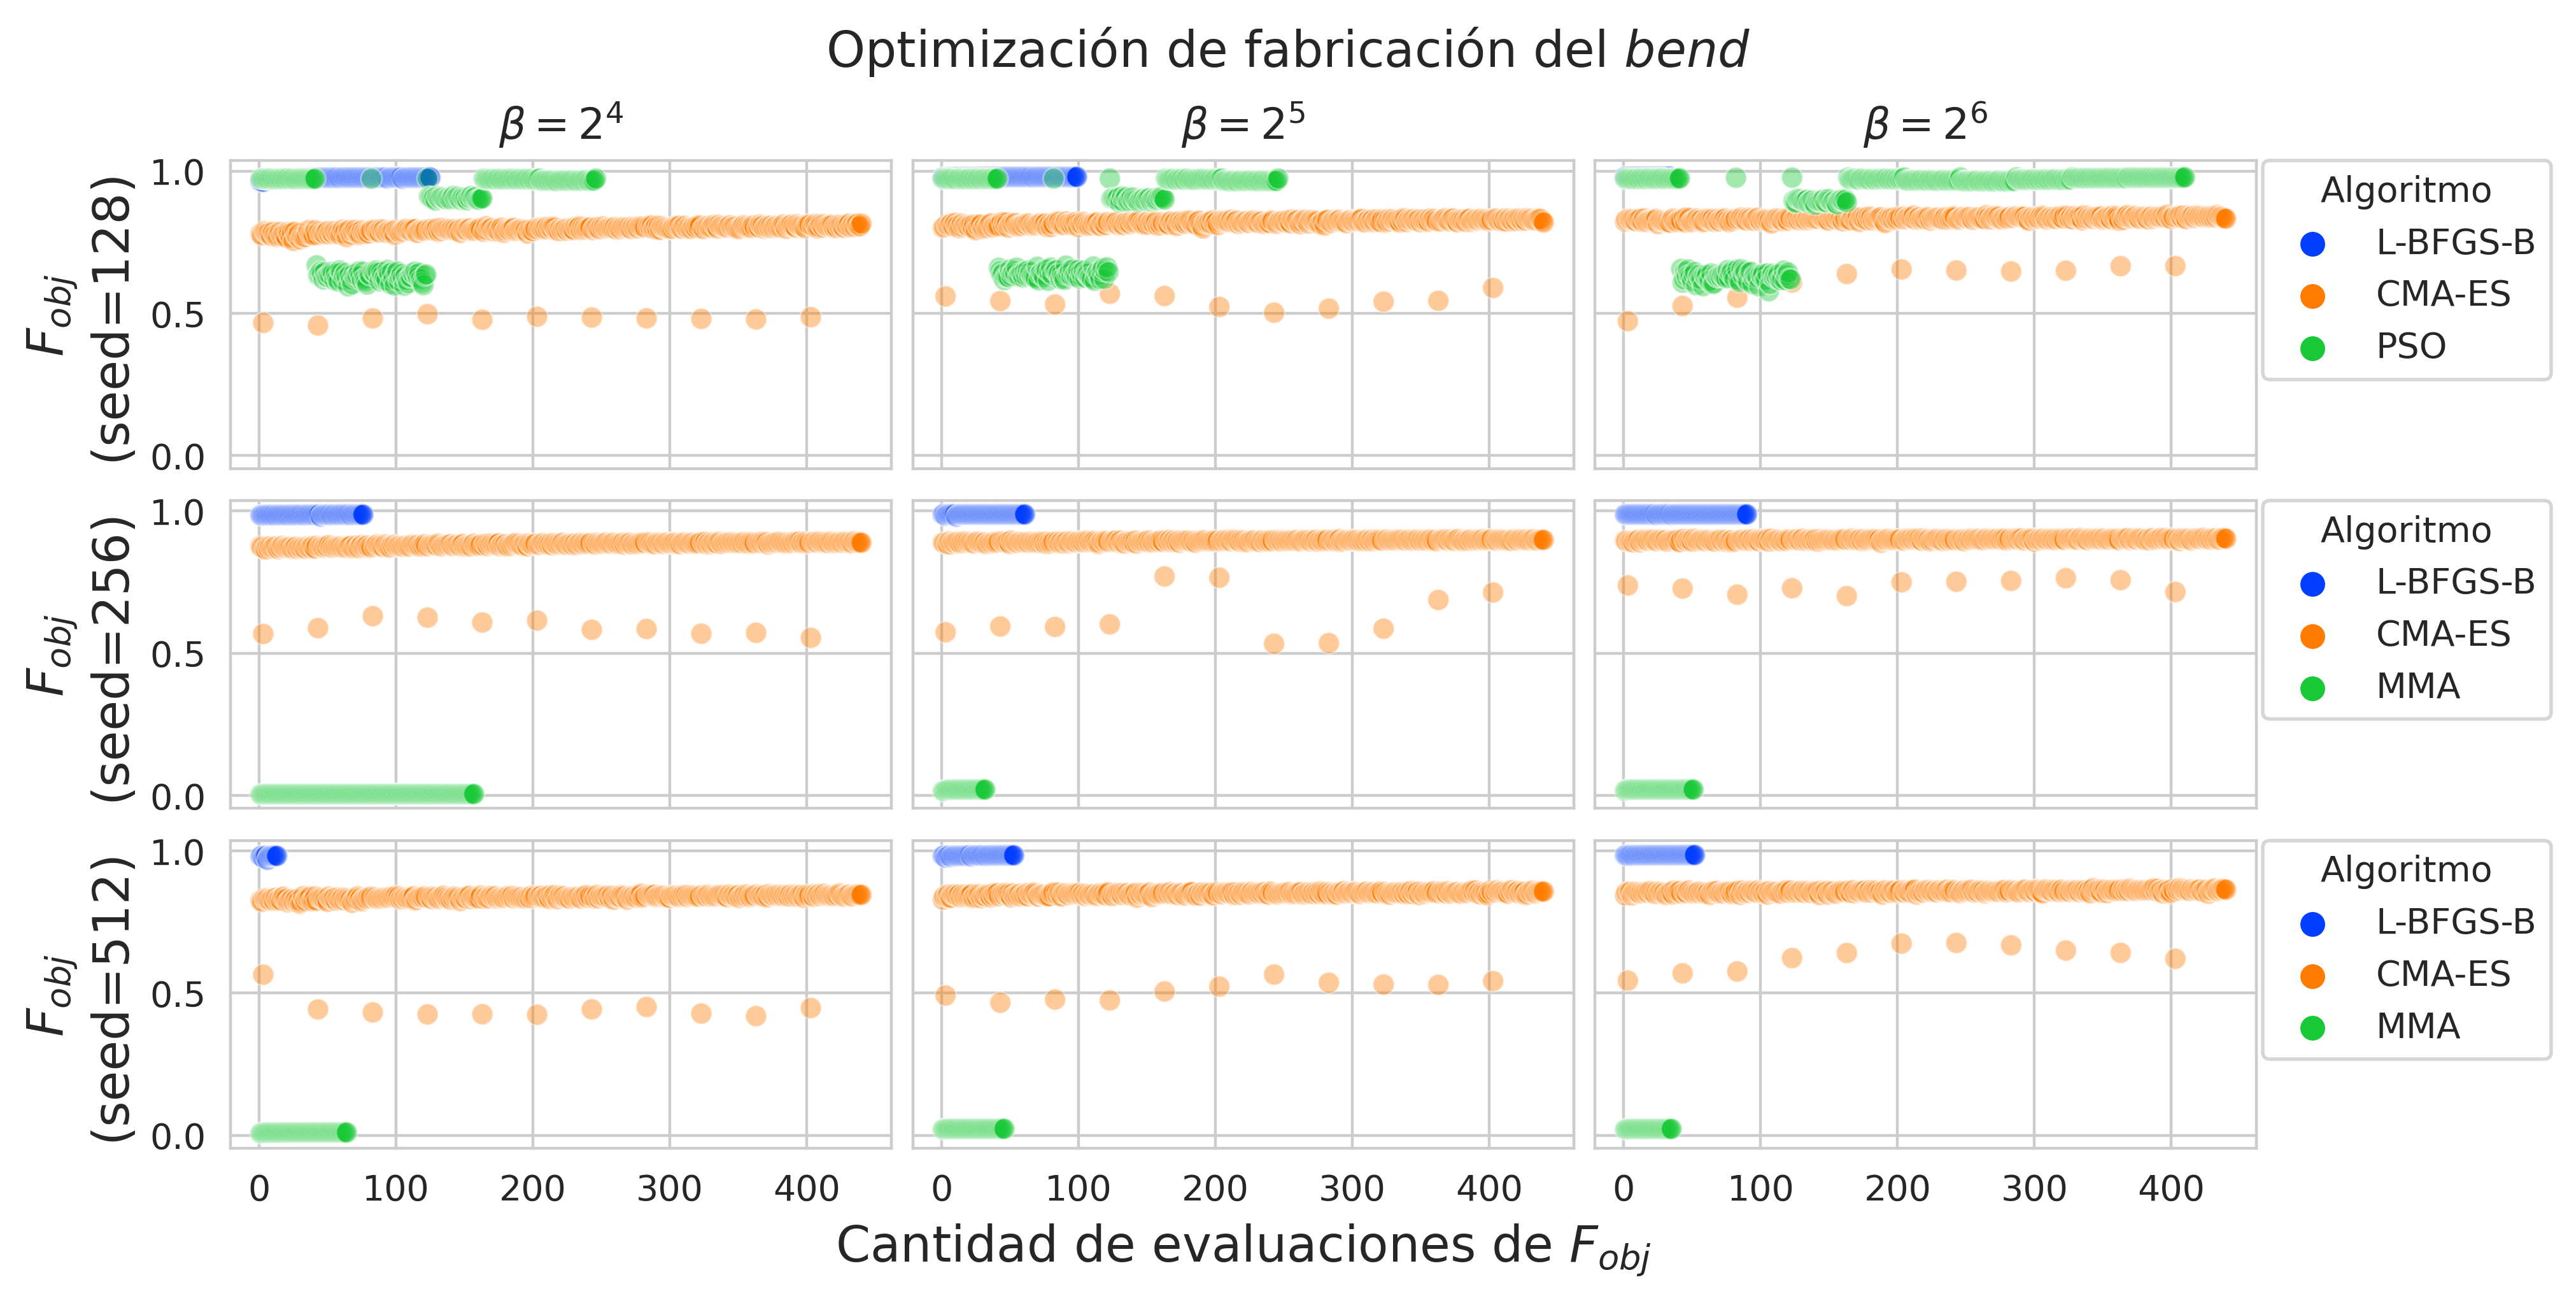
\includegraphics[scale=1.0]{image/results/bend/bend-opt-fab.png}
  \caption{Gráfico de valores de $F_{obj}$ obtenidos por los algoritmos en la optimización de fabricación del \emph{bend}}
  \label{fig:bend-fab}
\end{figure}
\end{landscape}

\begin{figure}[htp]
  \centering

  % 1° row
  \subfigure[Diseño nominal.]
  {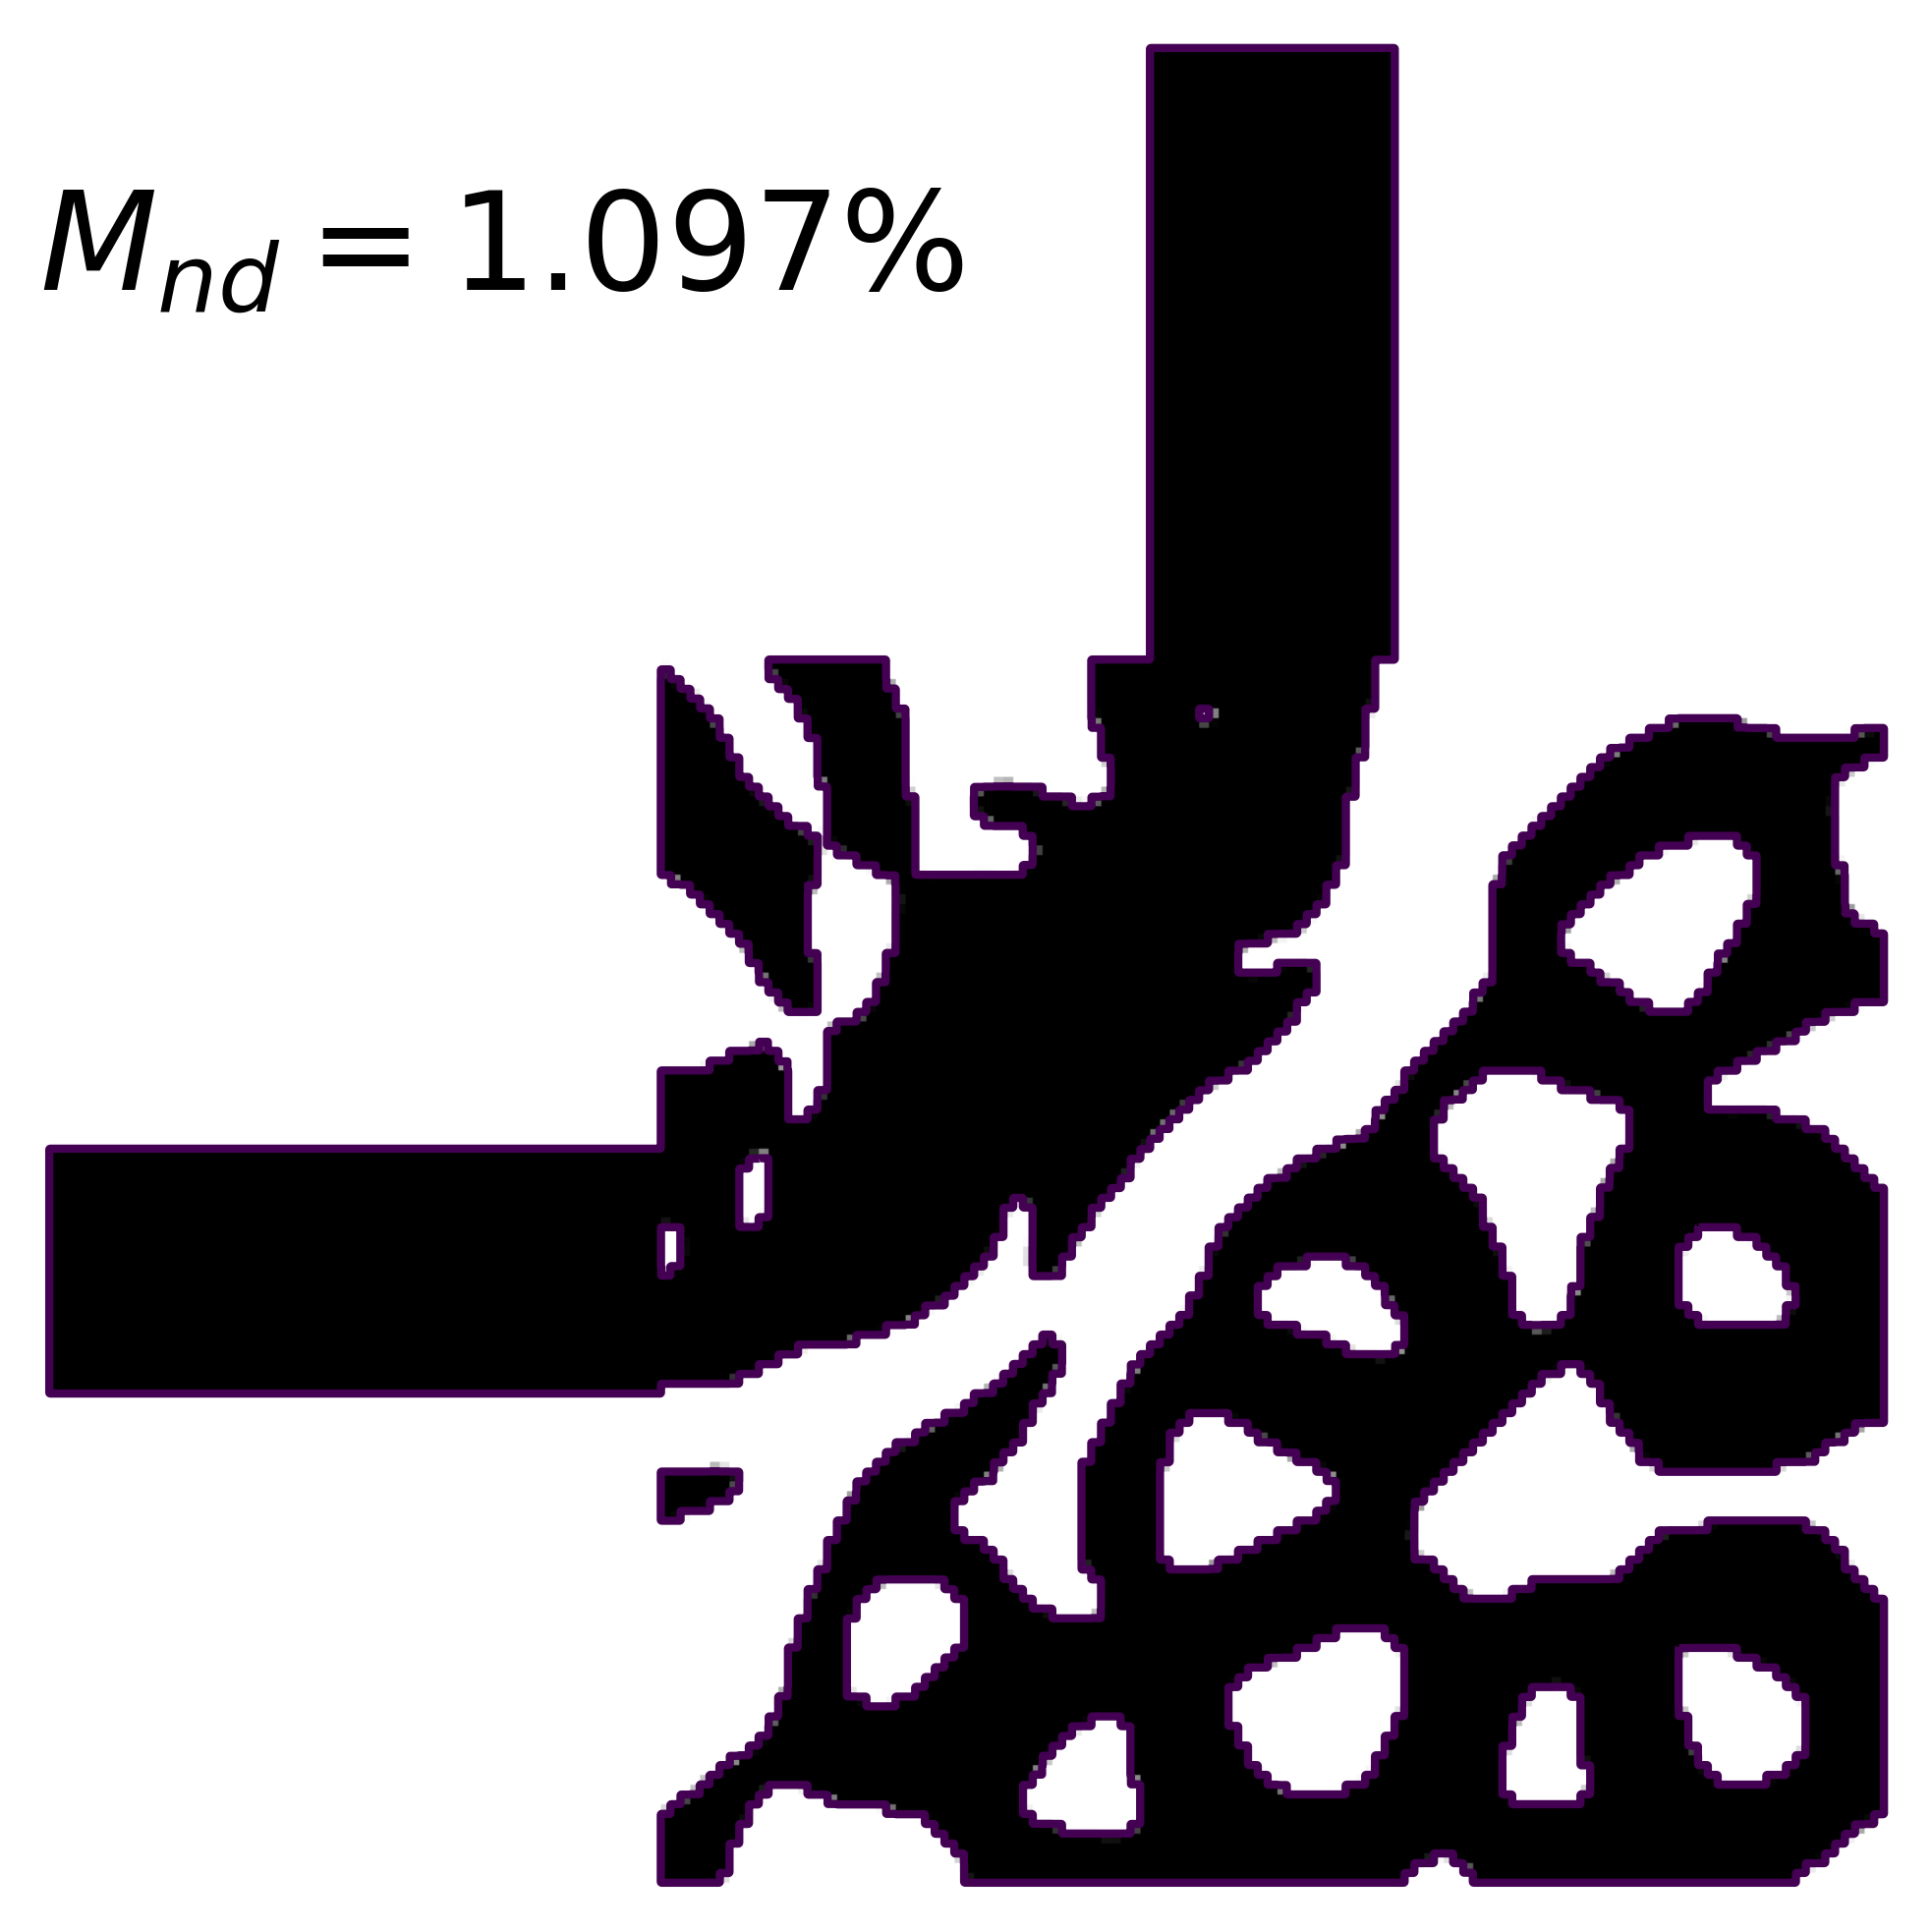
\includegraphics[width=0.40\textwidth]{image/results/bend/best/eps.png}}
  %\hfill
  \subfigure[Diseño nominal tras eliminar regiones no conexas.]
  {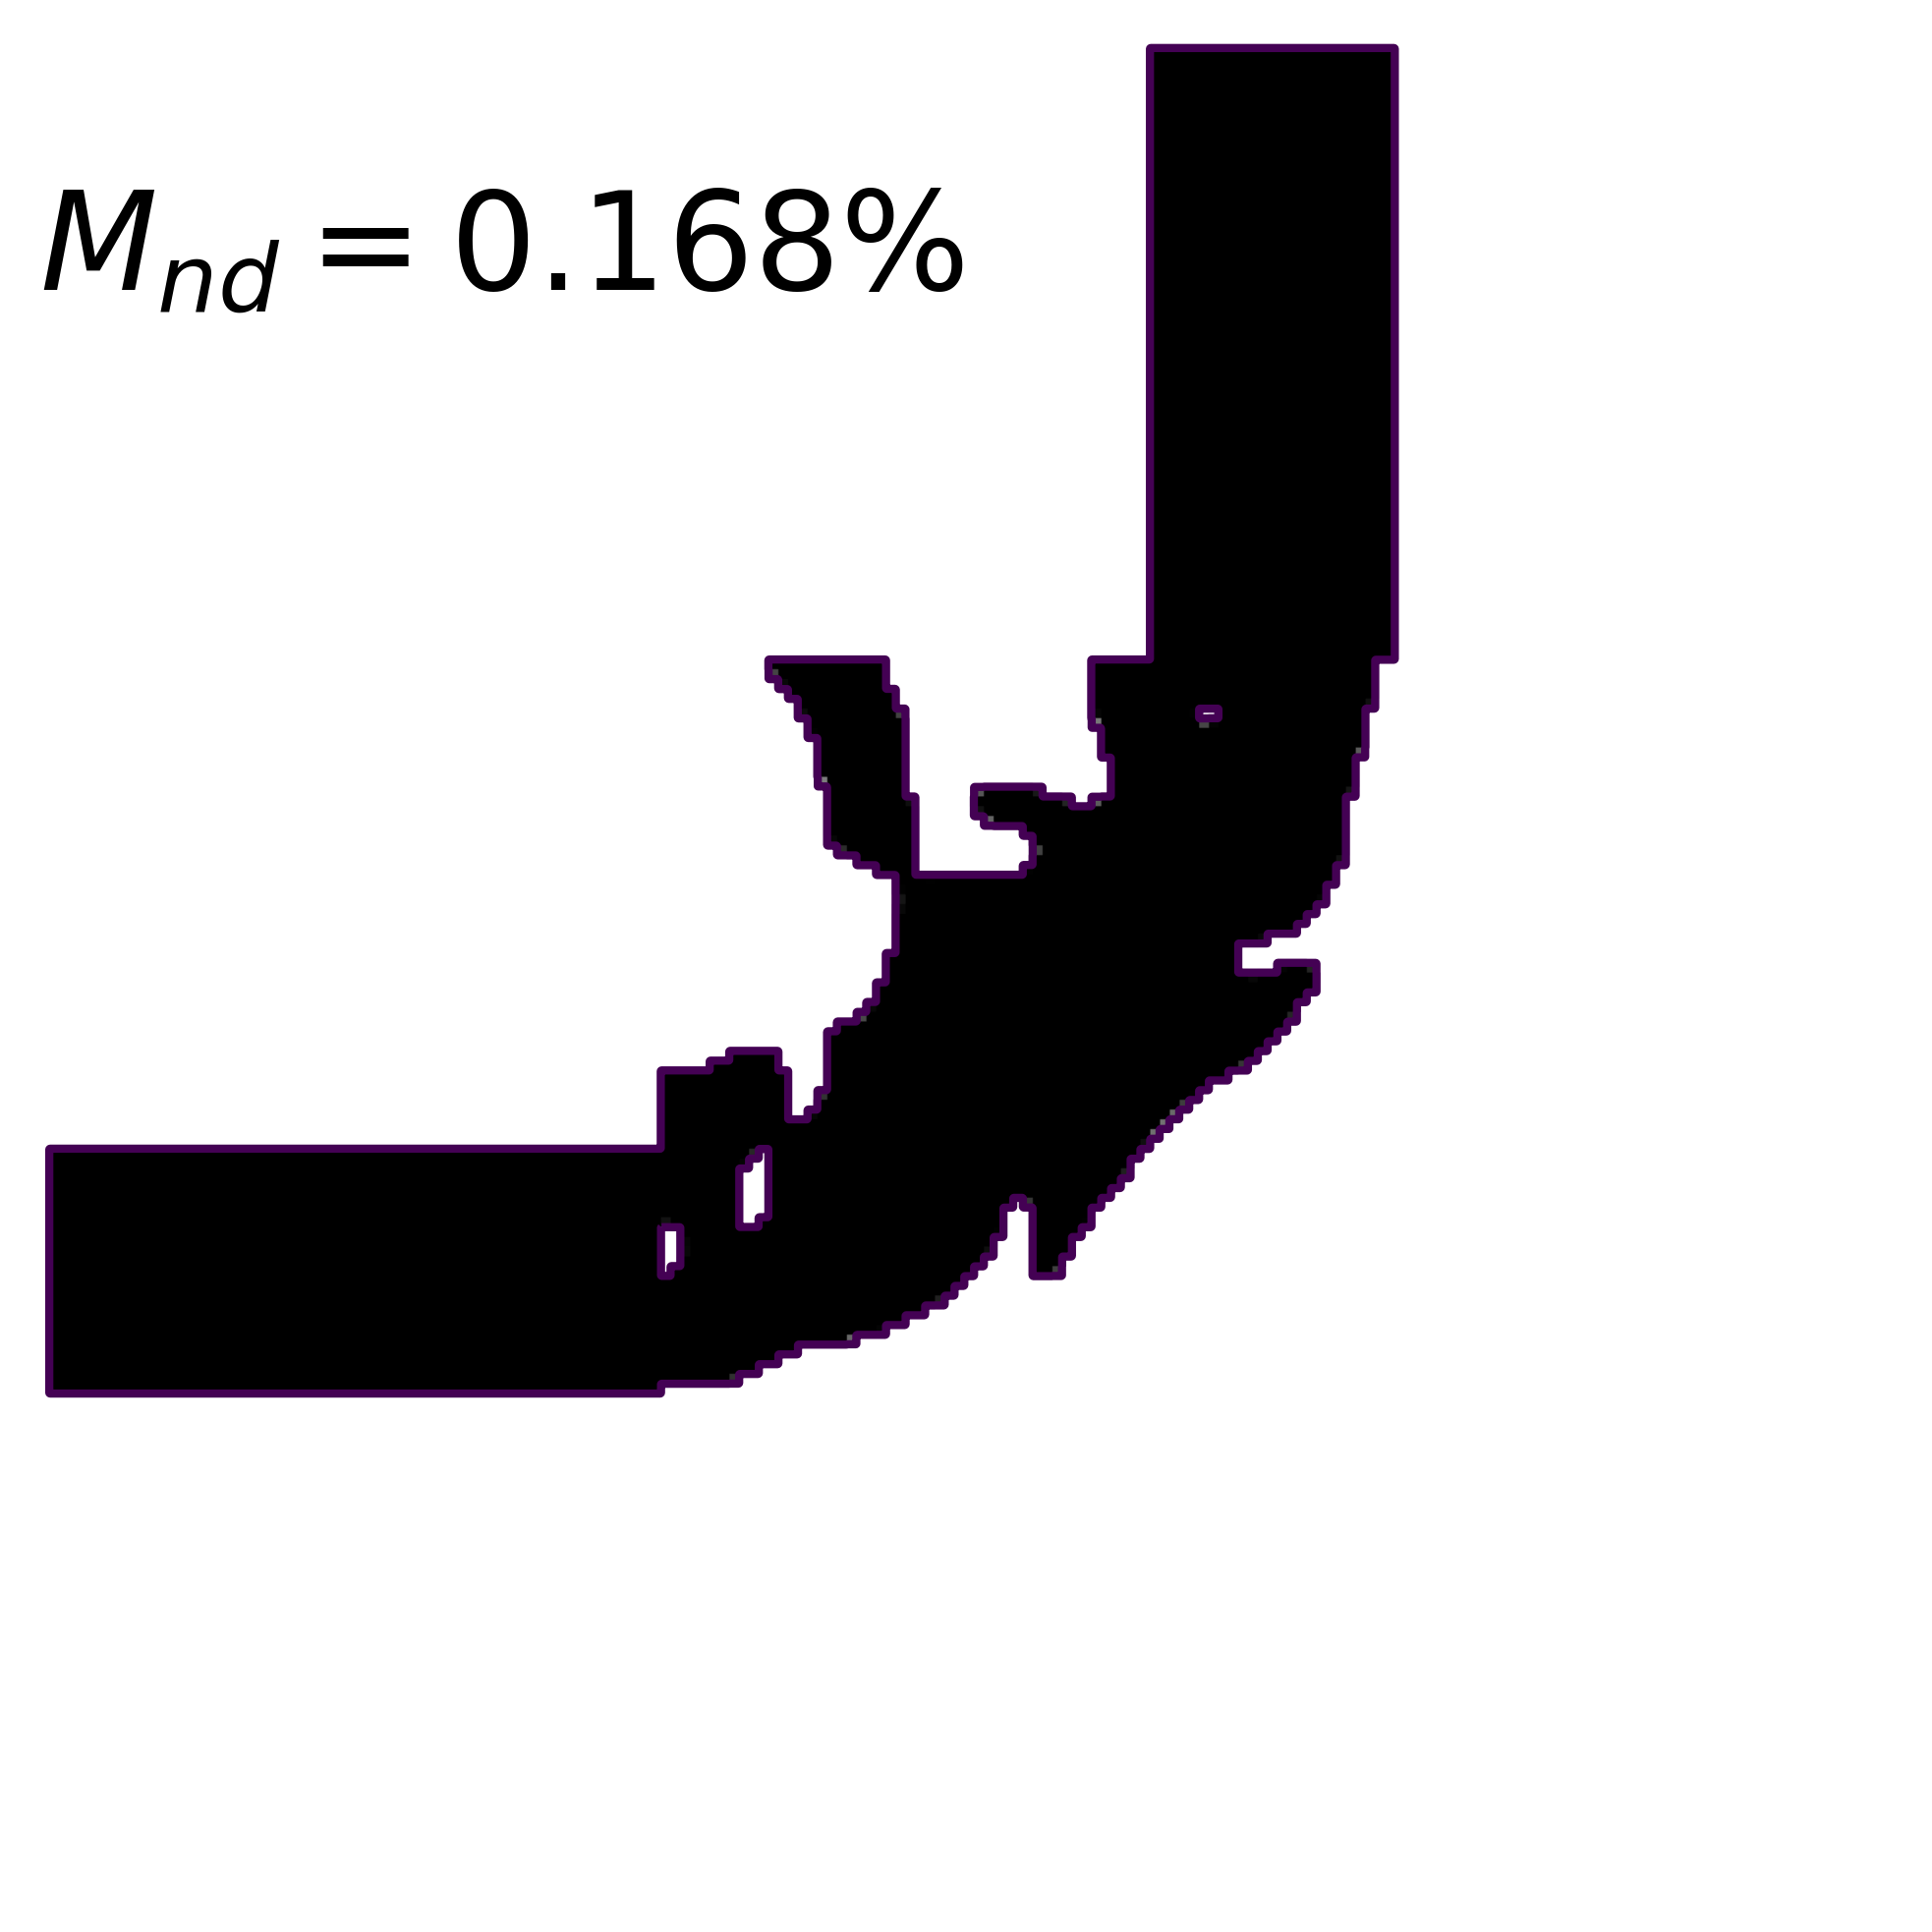
\includegraphics[width=0.40\textwidth]{image/results/bend/best/eps_post.png}}

  % 2° row
  \subfigure[Campo $|\boldsymbol{E}|^2$ del diseño nominal.]
  {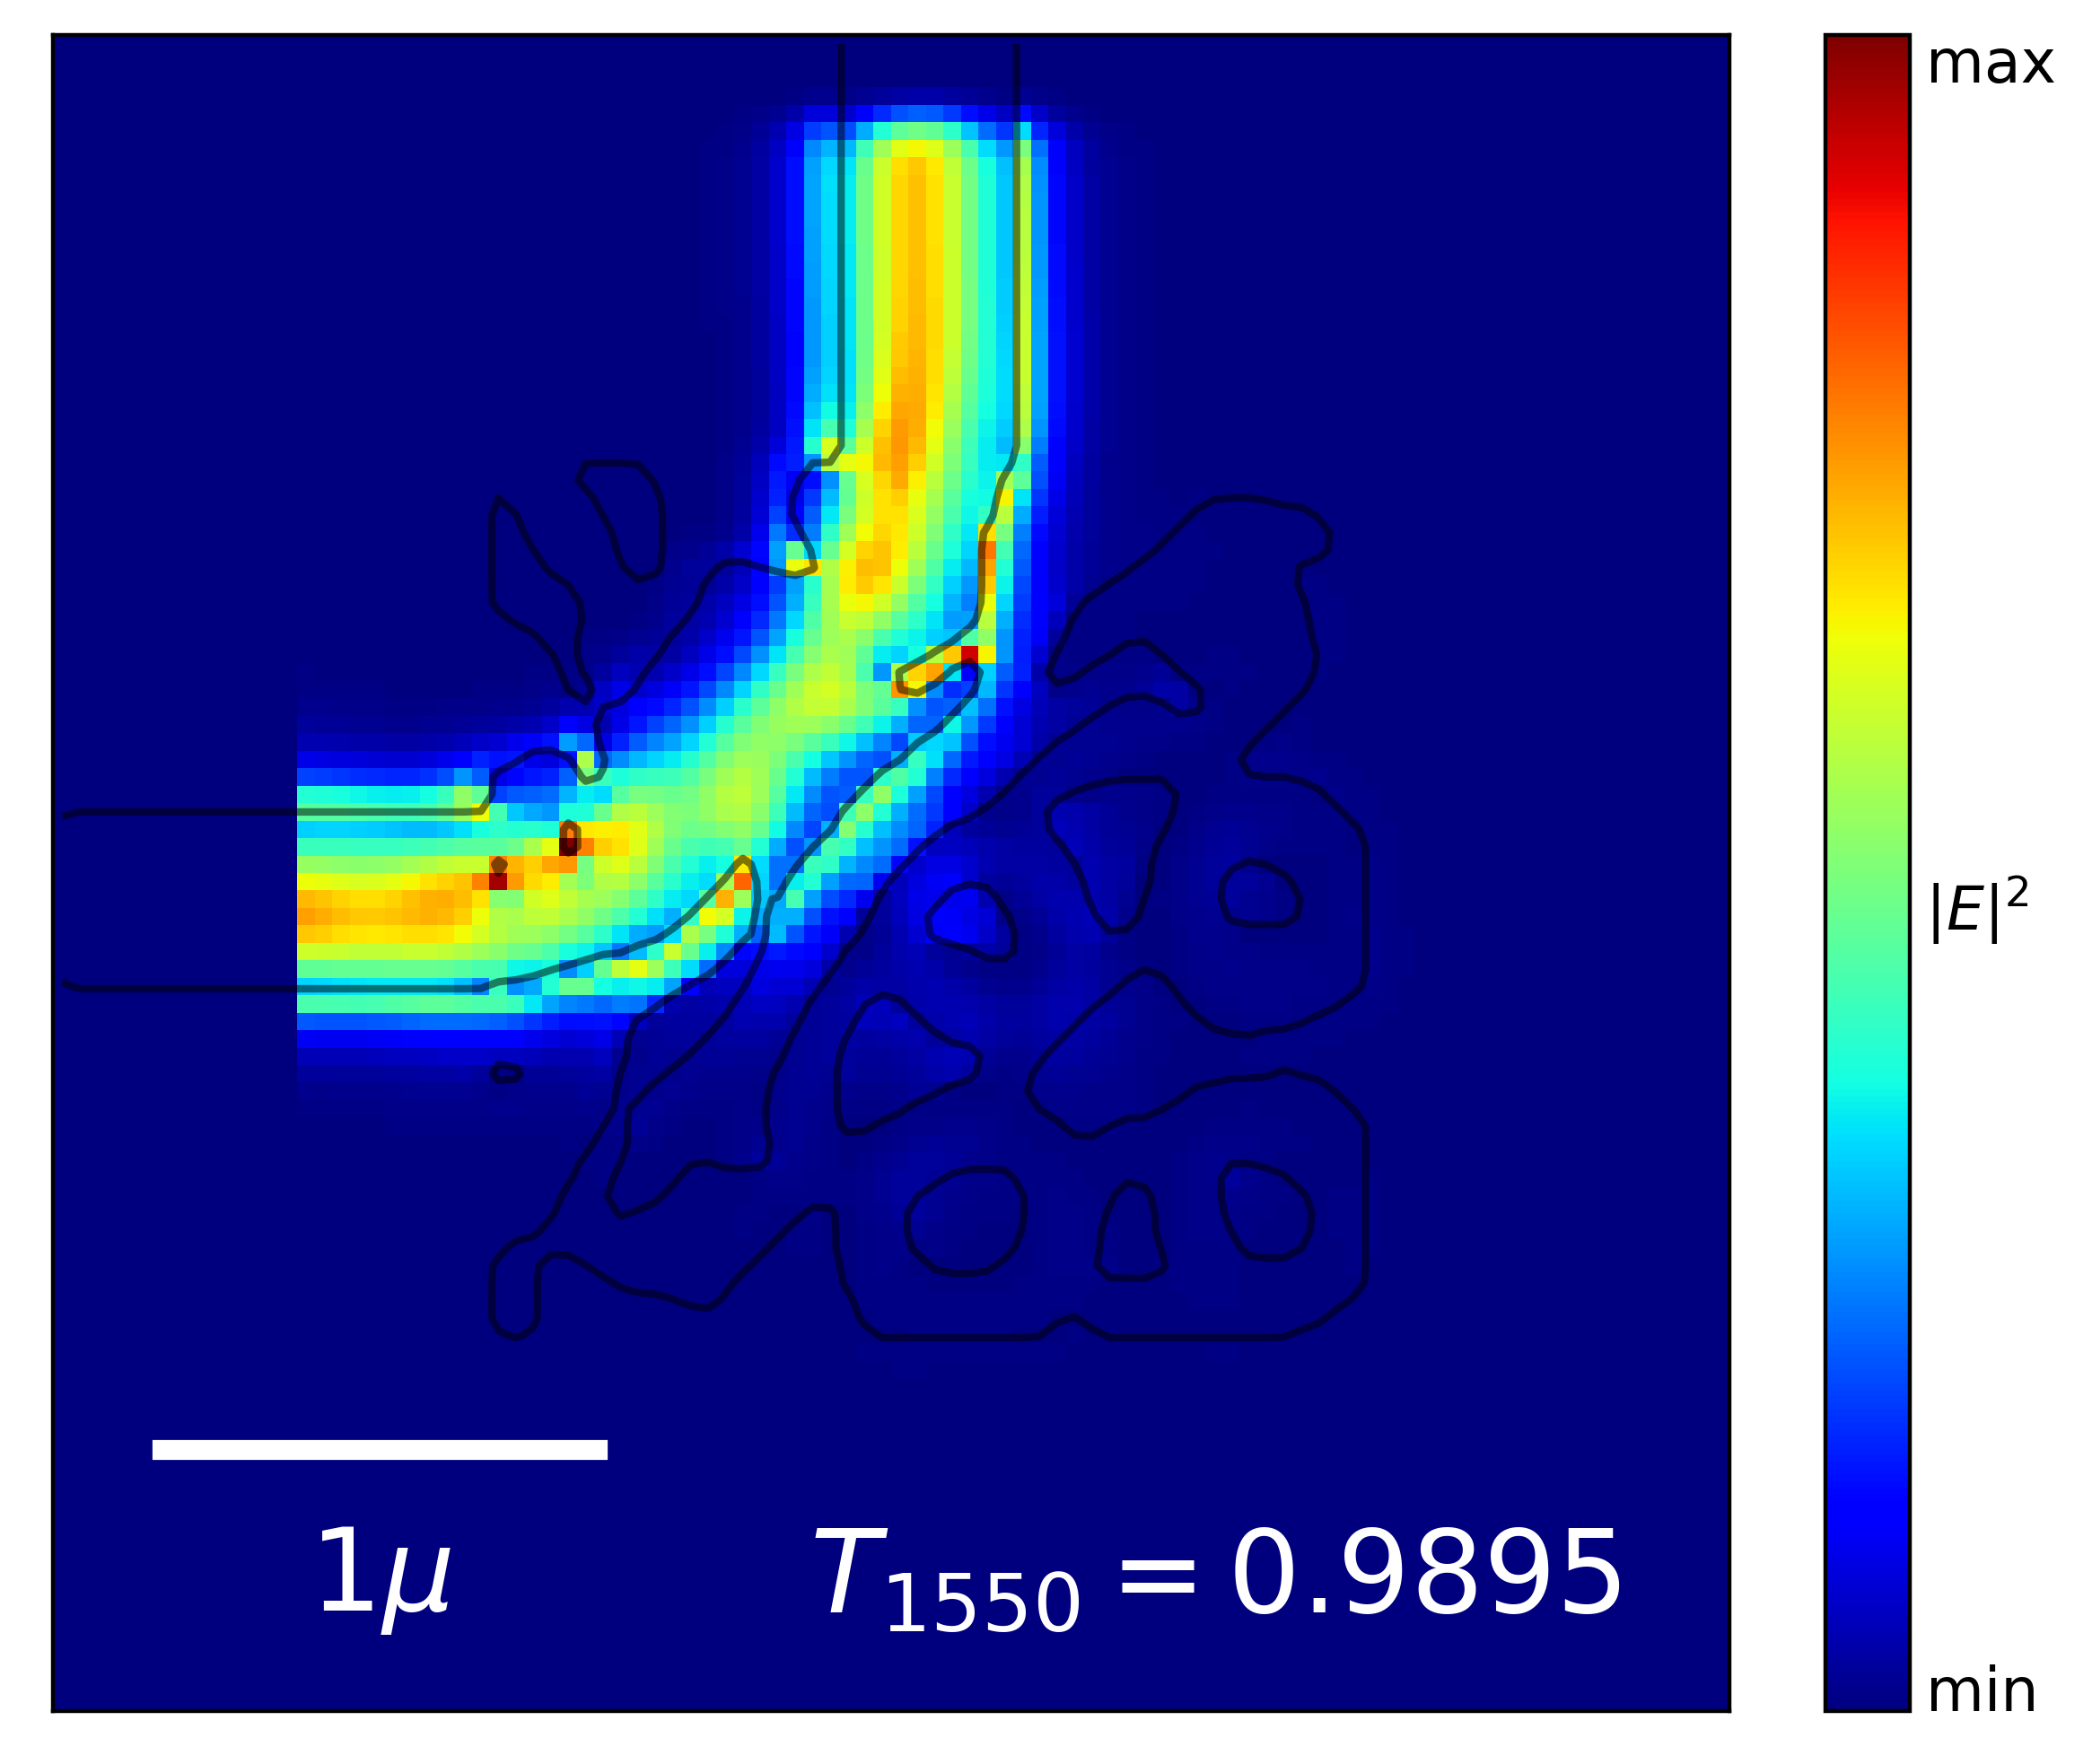
\includegraphics[width=0.40\textwidth]{image/results/bend/best/field.png}}
  %\hfill
  \subfigure[Campo $|\boldsymbol{E}|^2$ del diseño nominal tras eliminar regiones no conexas.]
  {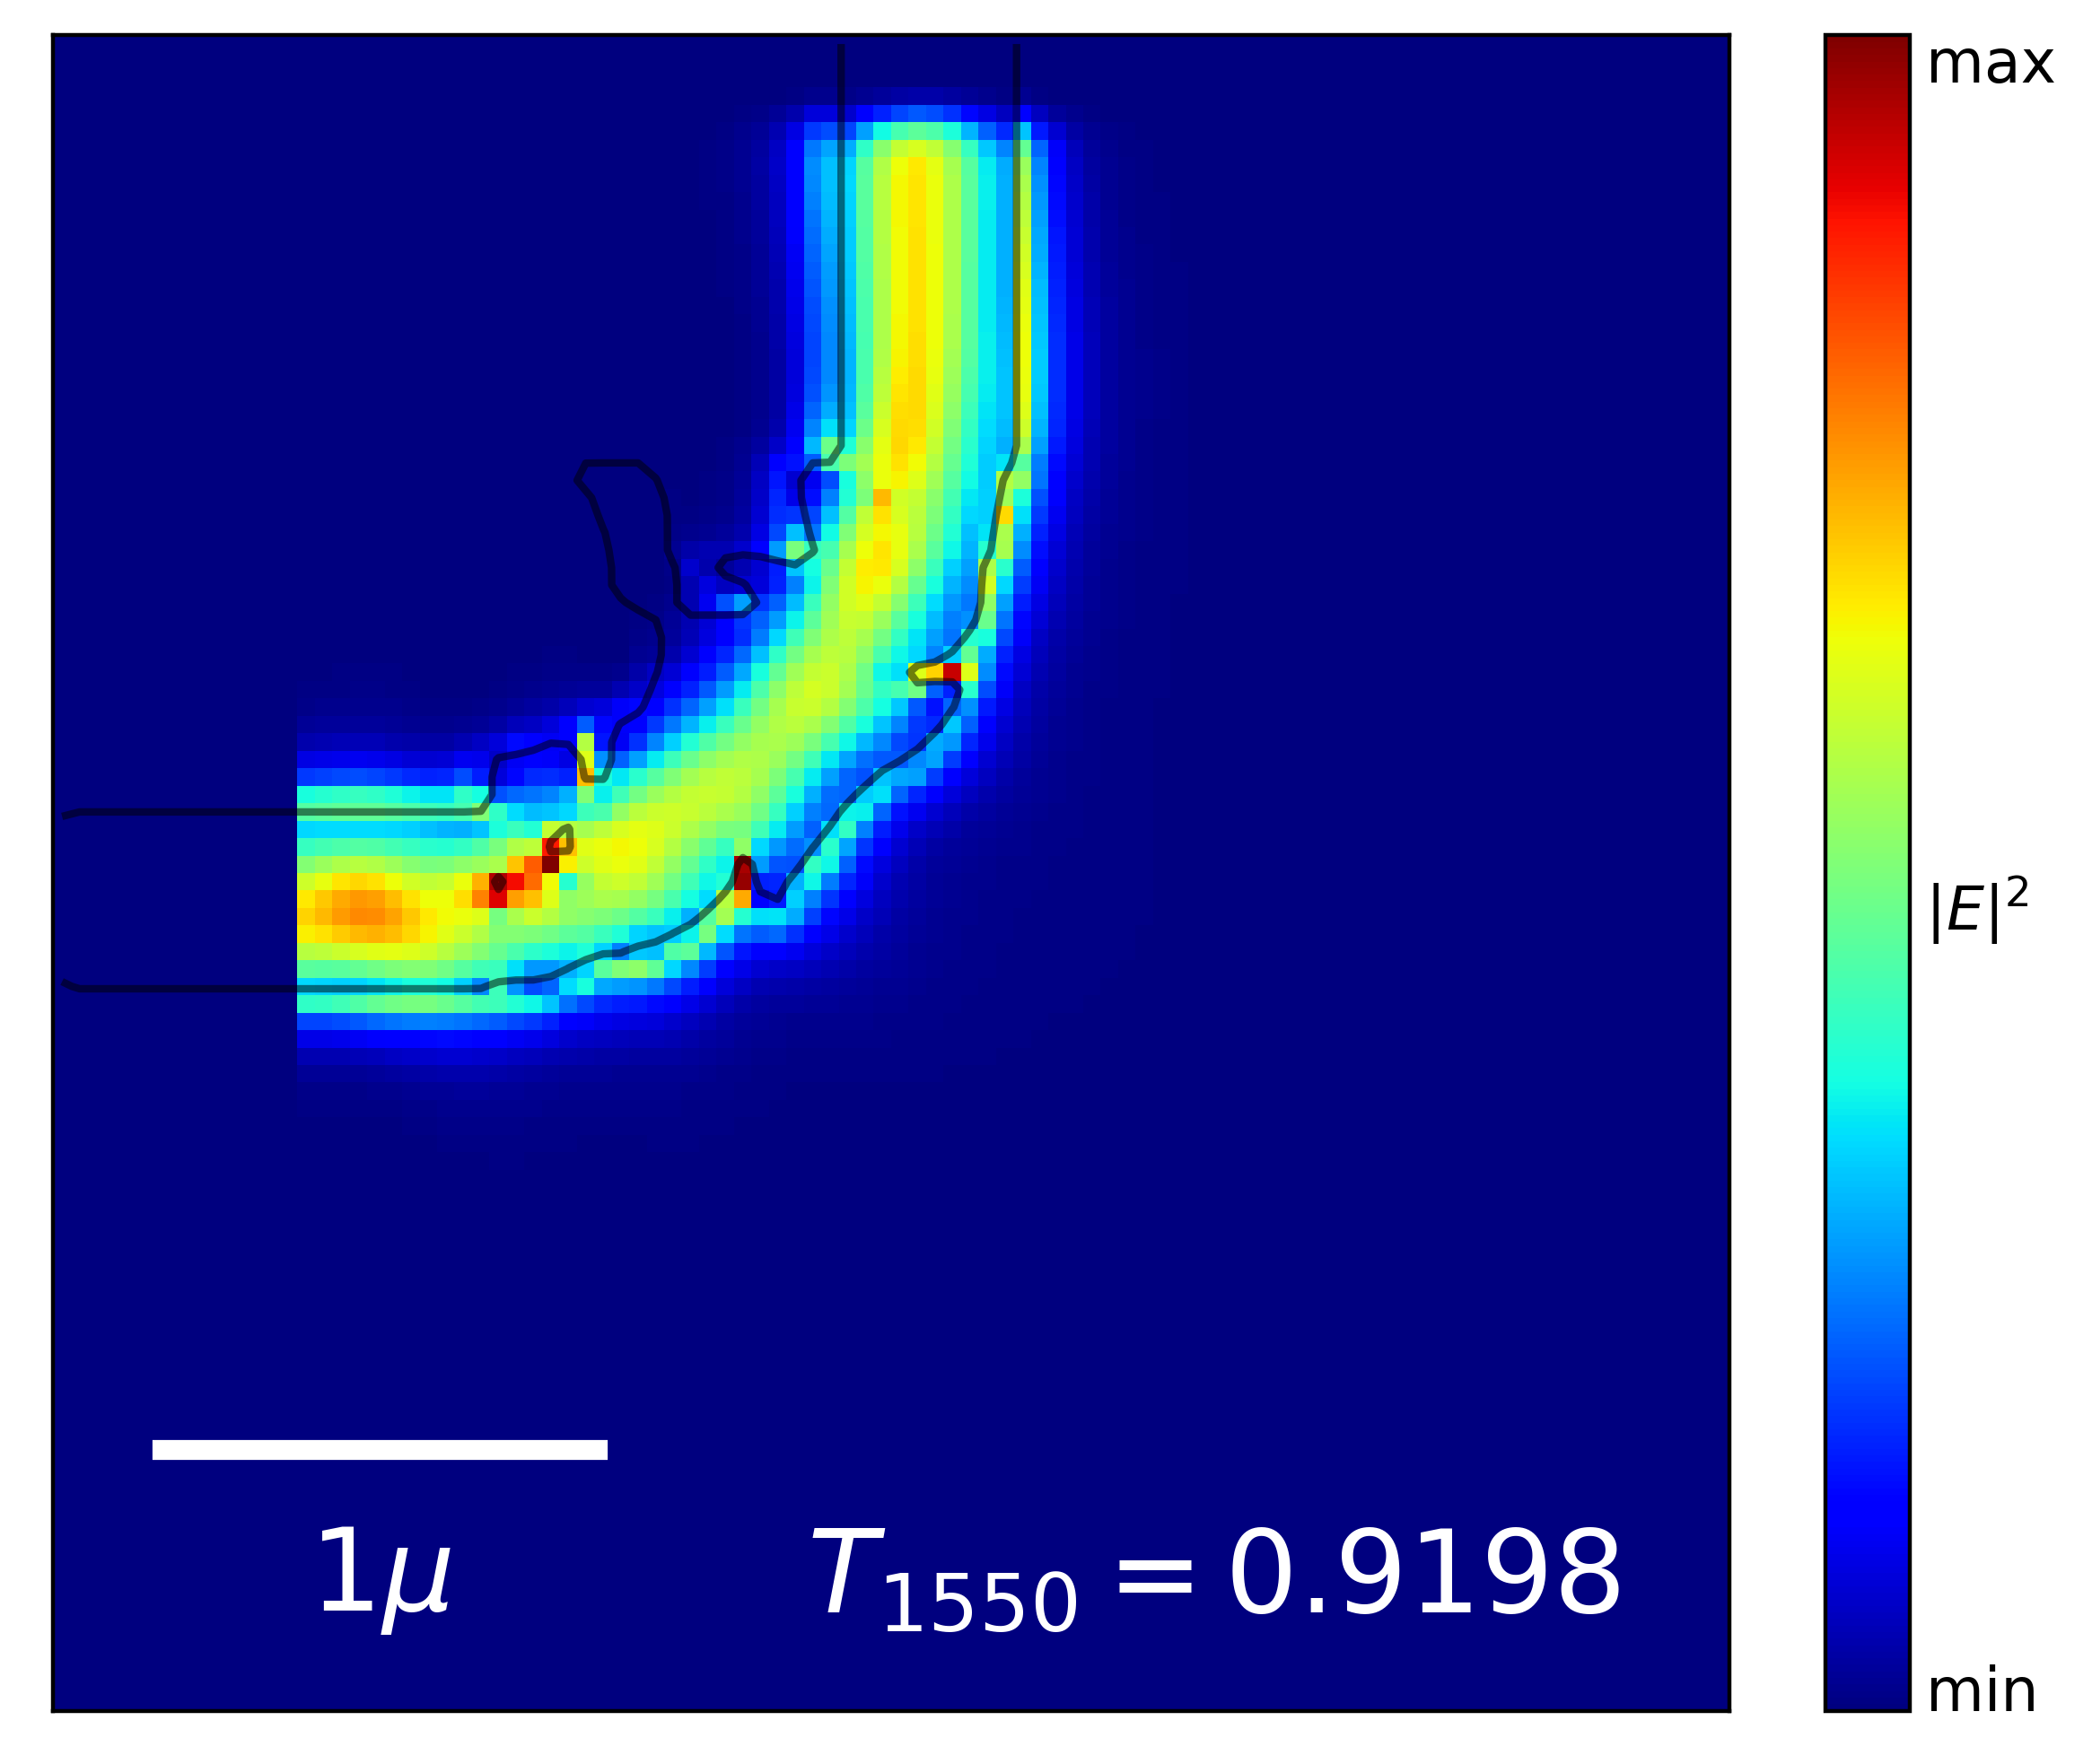
\includegraphics[width=0.40\textwidth]{image/results/bend/best/field_post.png}}

  % 3° row
  \subfigure[Representación GDSII del diseño nominal.]
  {\includesvg[width=0.40\textwidth]{image/results/bend/best/bend.svg}}
  %\hfill
  \subfigure[Representación GDSII del diseño nominal tras eliminar regiones no conexas.]
  {\includesvg[width=0.40\textwidth]{image/results/bend/best/bend_post.svg}}

  \caption{Posprocesamiento del diseño del \emph{bend} mejor optimizado.}
  \label{fig:bestbend}

\end{figure}

\section{Diseño del \emph{Bend} Mejor Optimizado}\label{sec:best-bend}

De la sección anterior tenemos que el \emph{bend} mejor optimizado se consiguió
utilizando el algoritmo L-BFGS-B con un \emph{seed} (valor de semilla) de 256.

Al aplicar la \autoref{eq:grayscale} obtenemos que el porcentaje de región gris en el diseño
es de 1.165 \%, un valor menor a 2 \%, por lo cual podemos considerar que el diseño ha sido
adecuadamente binarizado. 
Por otro lado, si eliminamos las regiones no conectadas con la guía de entrada
tenemos un diseño con un porcentaje de gris de 0.559 \%.
Estos diseños lo podemos observar en la \autoref{fig:bestbend}, 
el contorno morado alrededor de las geometrías de (a) y (b) representan los polígonos
usados para aproximar estas geometrías con el fin de obtener la descripción en el formato
GDSII, lo cual se puede observar en (e) y (f).
Adicionalmente, en la \autoref{fig:broadband-bend} se muestra el comportamiento del diseño
en un rango de longitudes de onda de $1500nm$ a $1600 nm$, resultados obtenidos usando una ventana de $50nm$.
En este rango, considerando los errores de erosión y dilatación, 
la máxima diferencia de transmitancia es de 0.032 para el diseño nominal
y de 0.034 para el diseño nominal tras eliminar regiones no conexas.

\begin{figure}[H]
  \centering
  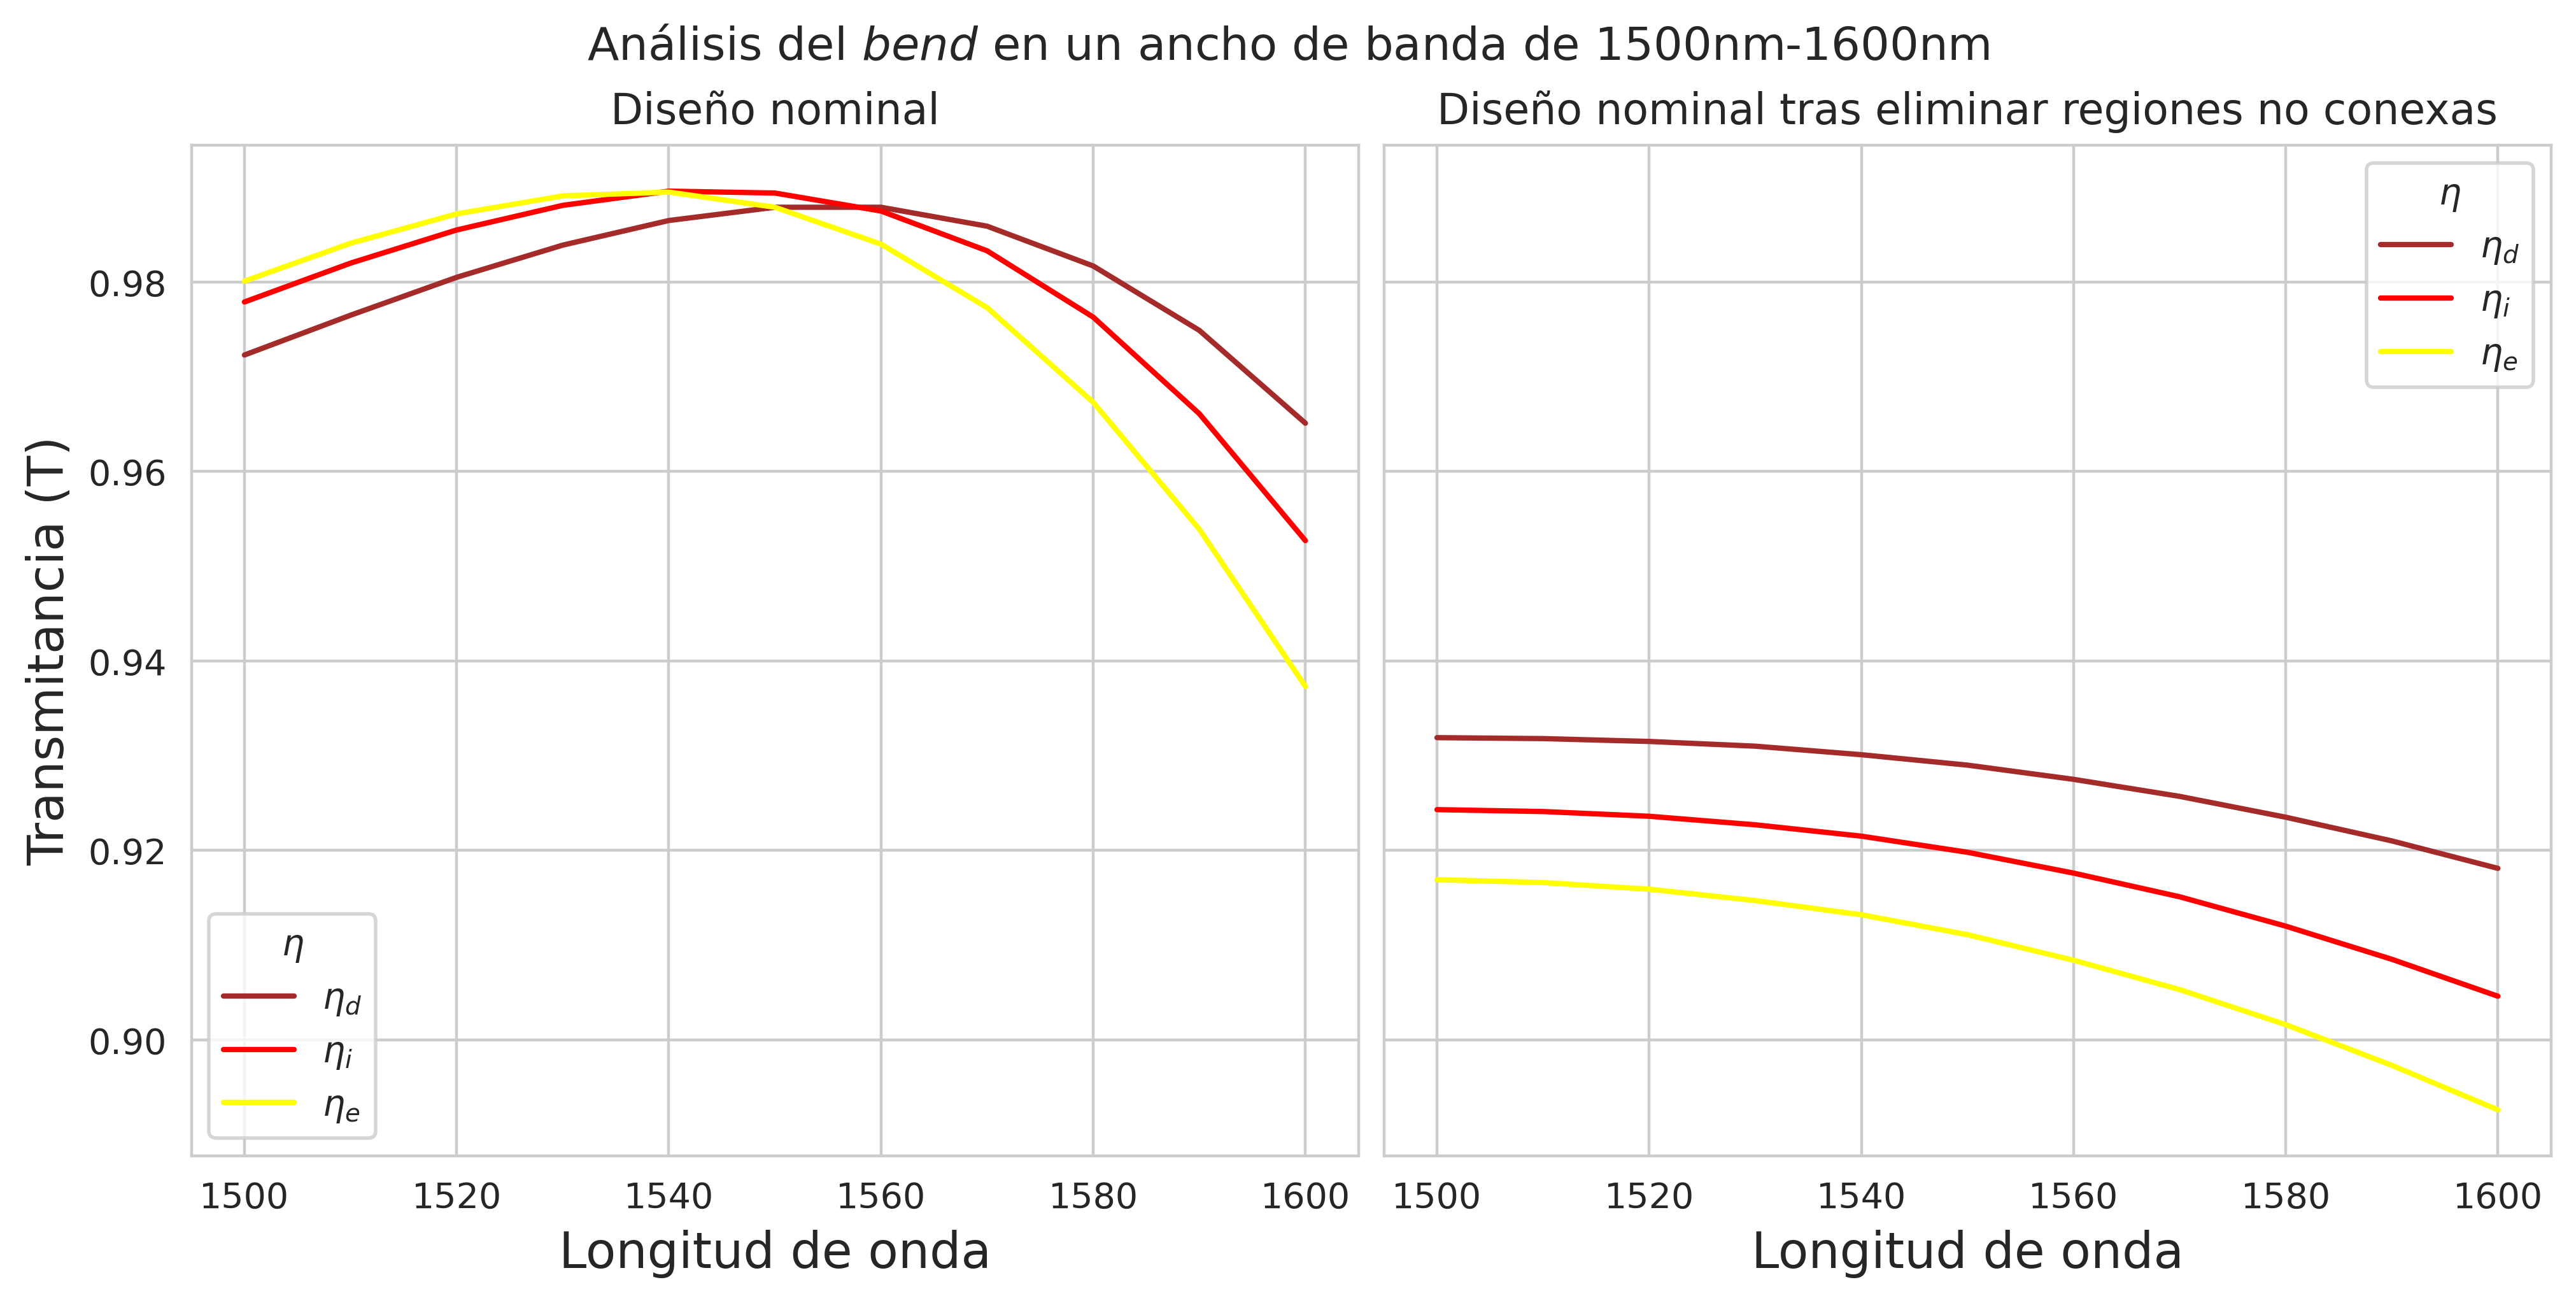
\includegraphics[width=0.95\textwidth]{image/results/bend/best/broadband-bend.png}
  \caption{Análisis del \emph{bend} mejor optimizado en un rango de longitudes de onda ($1500 nm-1600 nm$)}
  \label{fig:broadband-bend}
\end{figure}


\section{Resultados de Optimización del WDM}\label{sec:results-wdm}

En la \autoref{fig:wdm-cont}, \autoref{fig:wdm-disc} y \autoref{fig:wdm-fab} se observa 
el desempeño de los cinco algoritmos seleccionados en la etapa de optimización continua, discreta y
de fabricación del WDM, respectivamente.
Los resultados en más detalle por algoritmo se pueden encontrar en la
\autoref{tab:opt-LBFGSB-wdm} (L-BFGS-B),
\autoref{tab:opt-CMA-wdm} (G-CMA-ES),
\autoref{tab:opt-MMA-wdm} (MMA),
\autoref{tab:opt-PSO-wdm} (G-PSO) y
\autoref{tab:opt-GA-wdm} (G-GA).

\begin{landscape}
\begin{figure}[ht]
  \centering
  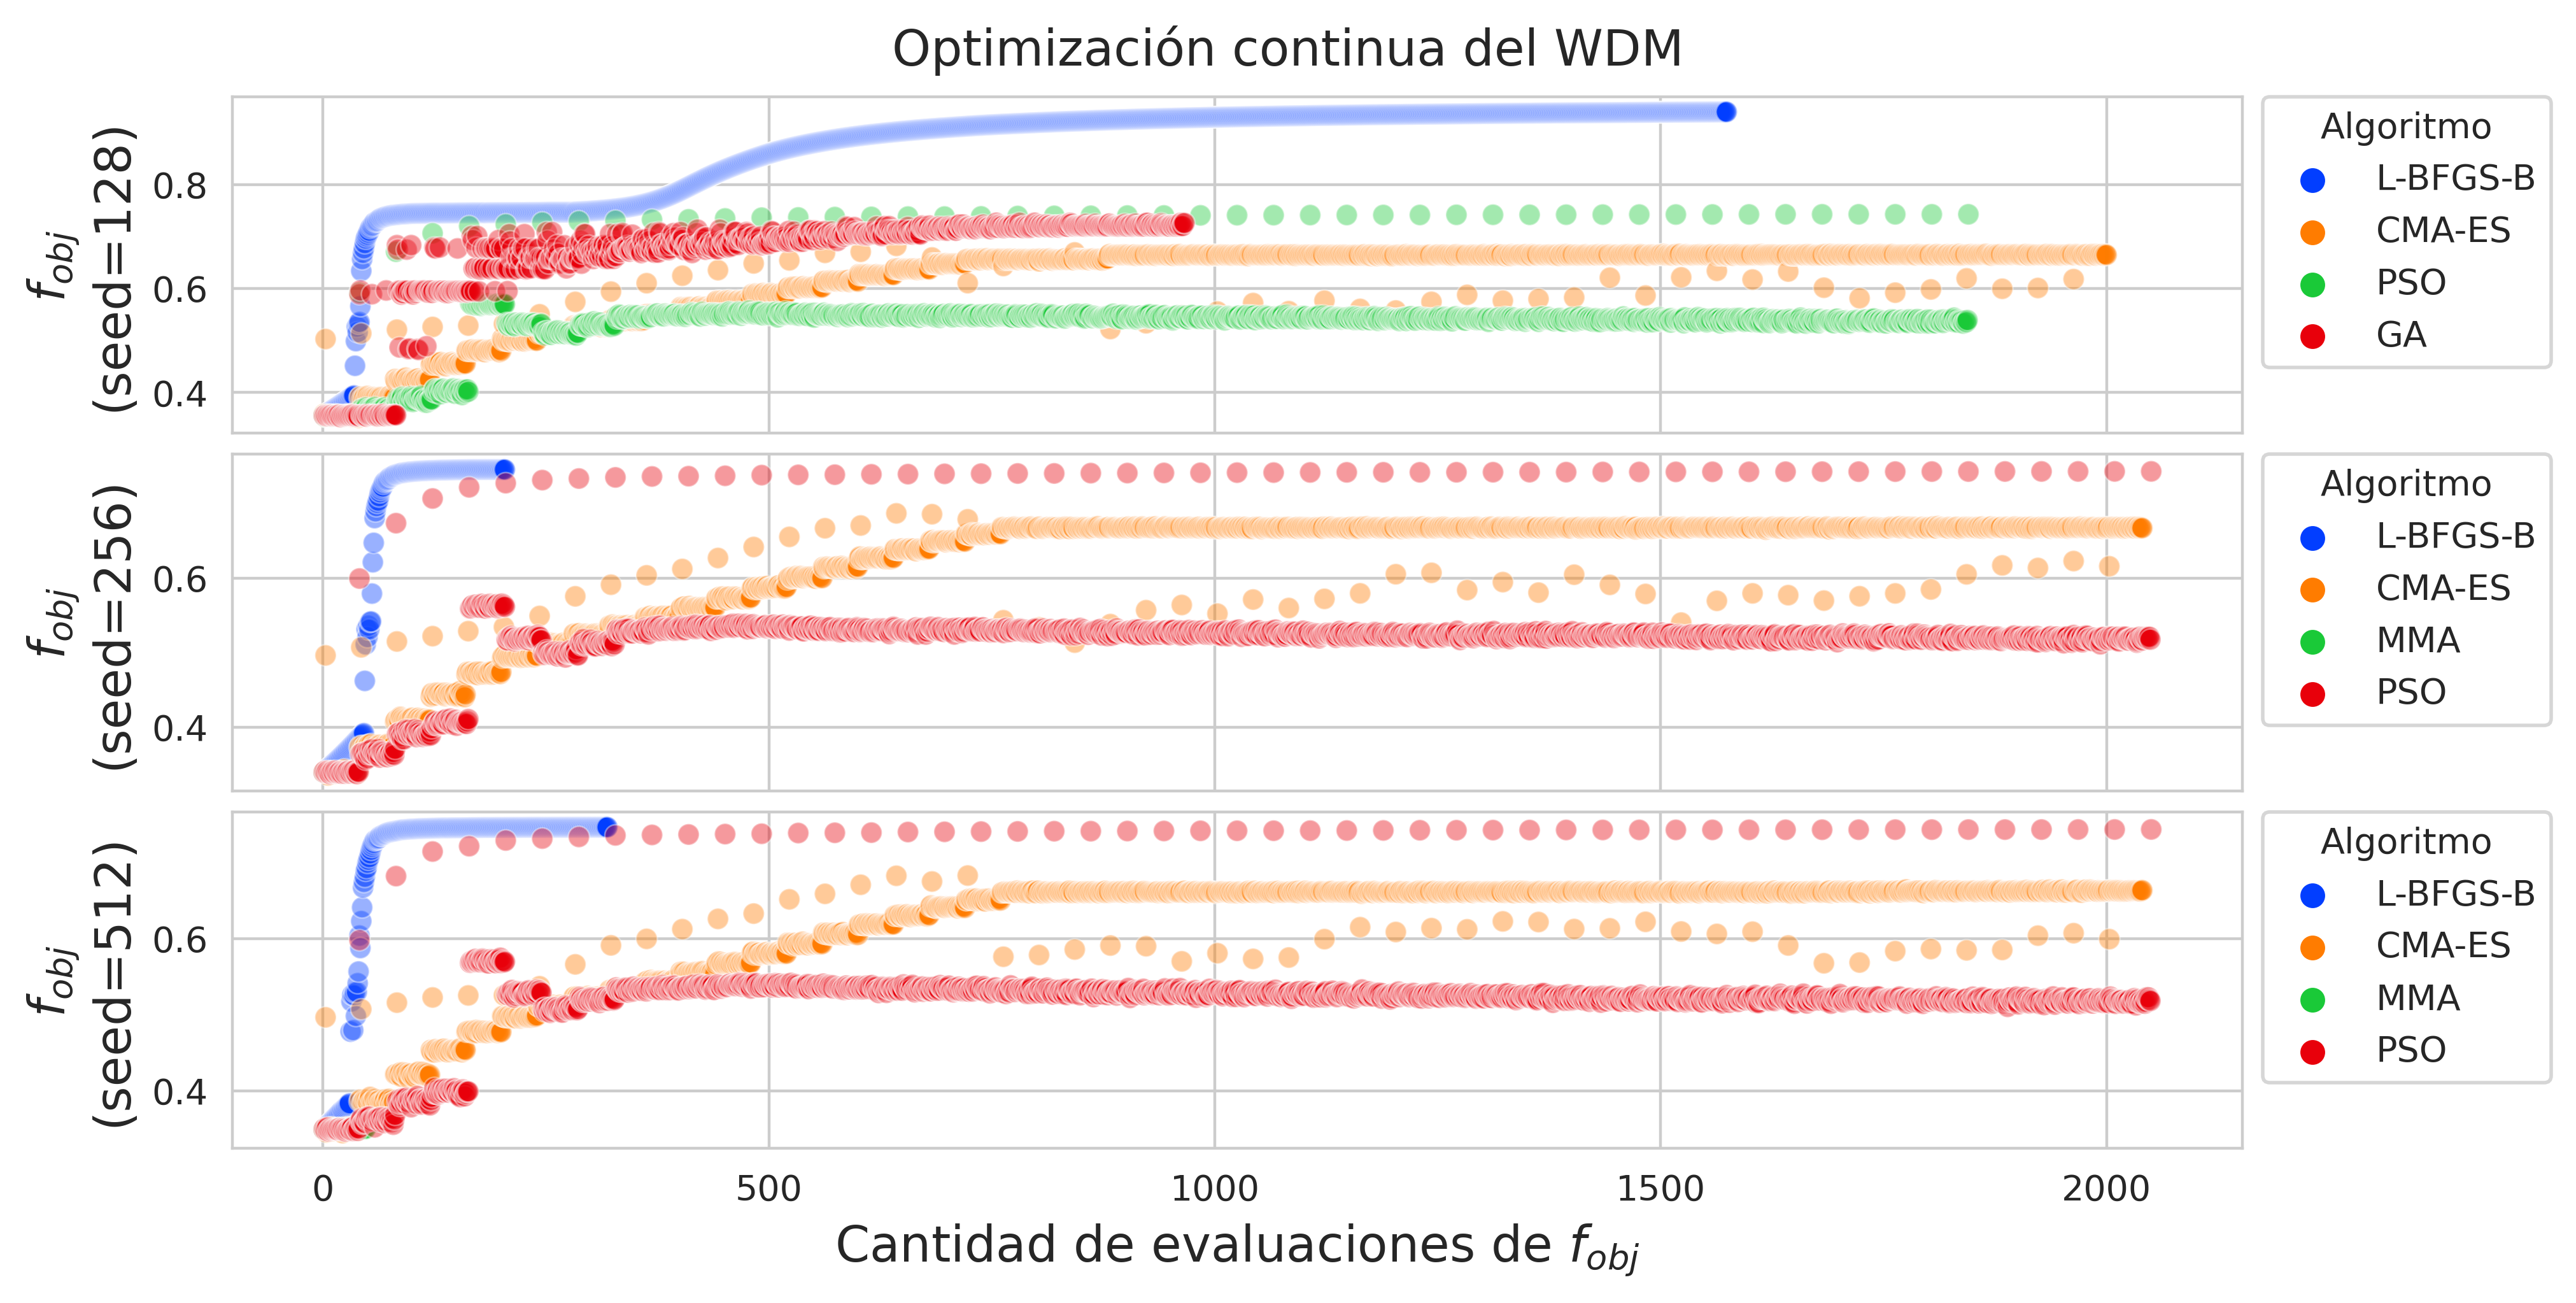
\includegraphics[scale=1.0]{image/results/wdm/wdm-opt-cont.png}
  \caption{Gráfico de valores de $f_{obj}$ obtenidos por los algoritmos en la optimización continua del WDM}
  \label{fig:wdm-cont}
\end{figure}
\end{landscape}

\begin{landscape}
\begin{figure}[ht]
  \centering
  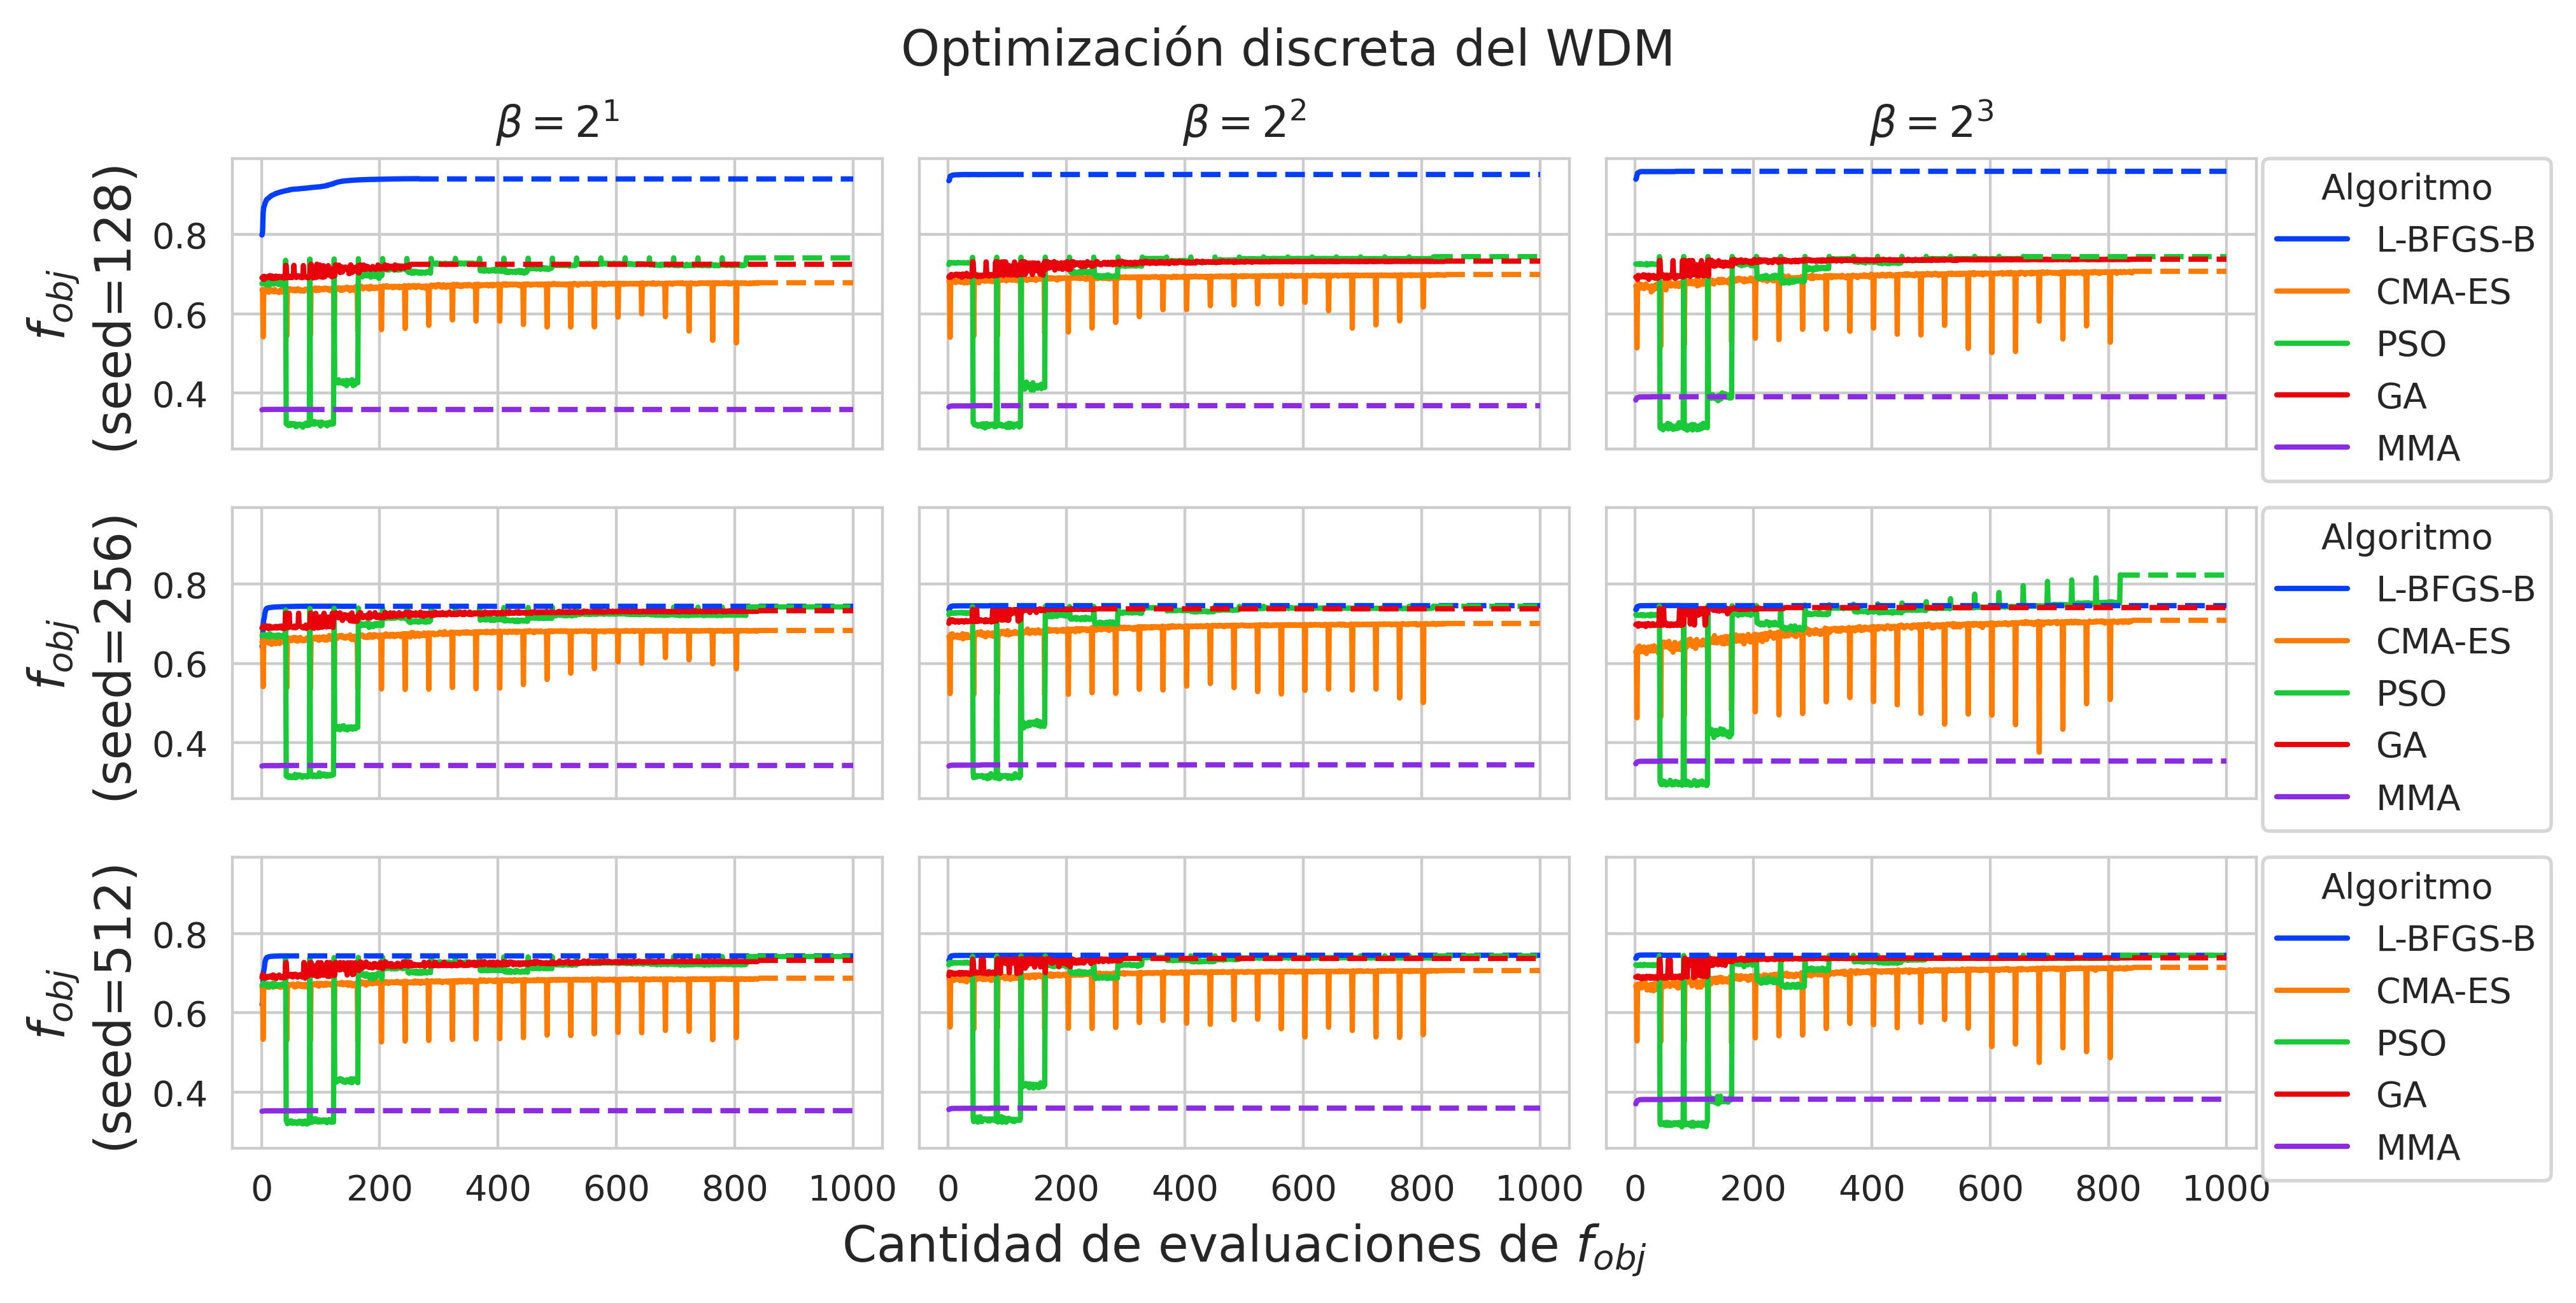
\includegraphics[scale=1.0]{image/results/wdm/wdm-opt-disc.png}
  \caption{Gráfico de valores de $f_{obj}$ obtenidos por los algoritmos en la optimización discreta del WDM}
  \label{fig:wdm-disc}
\end{figure}
\end{landscape}

\begin{landscape}
\begin{figure}[ht]
  \centering
  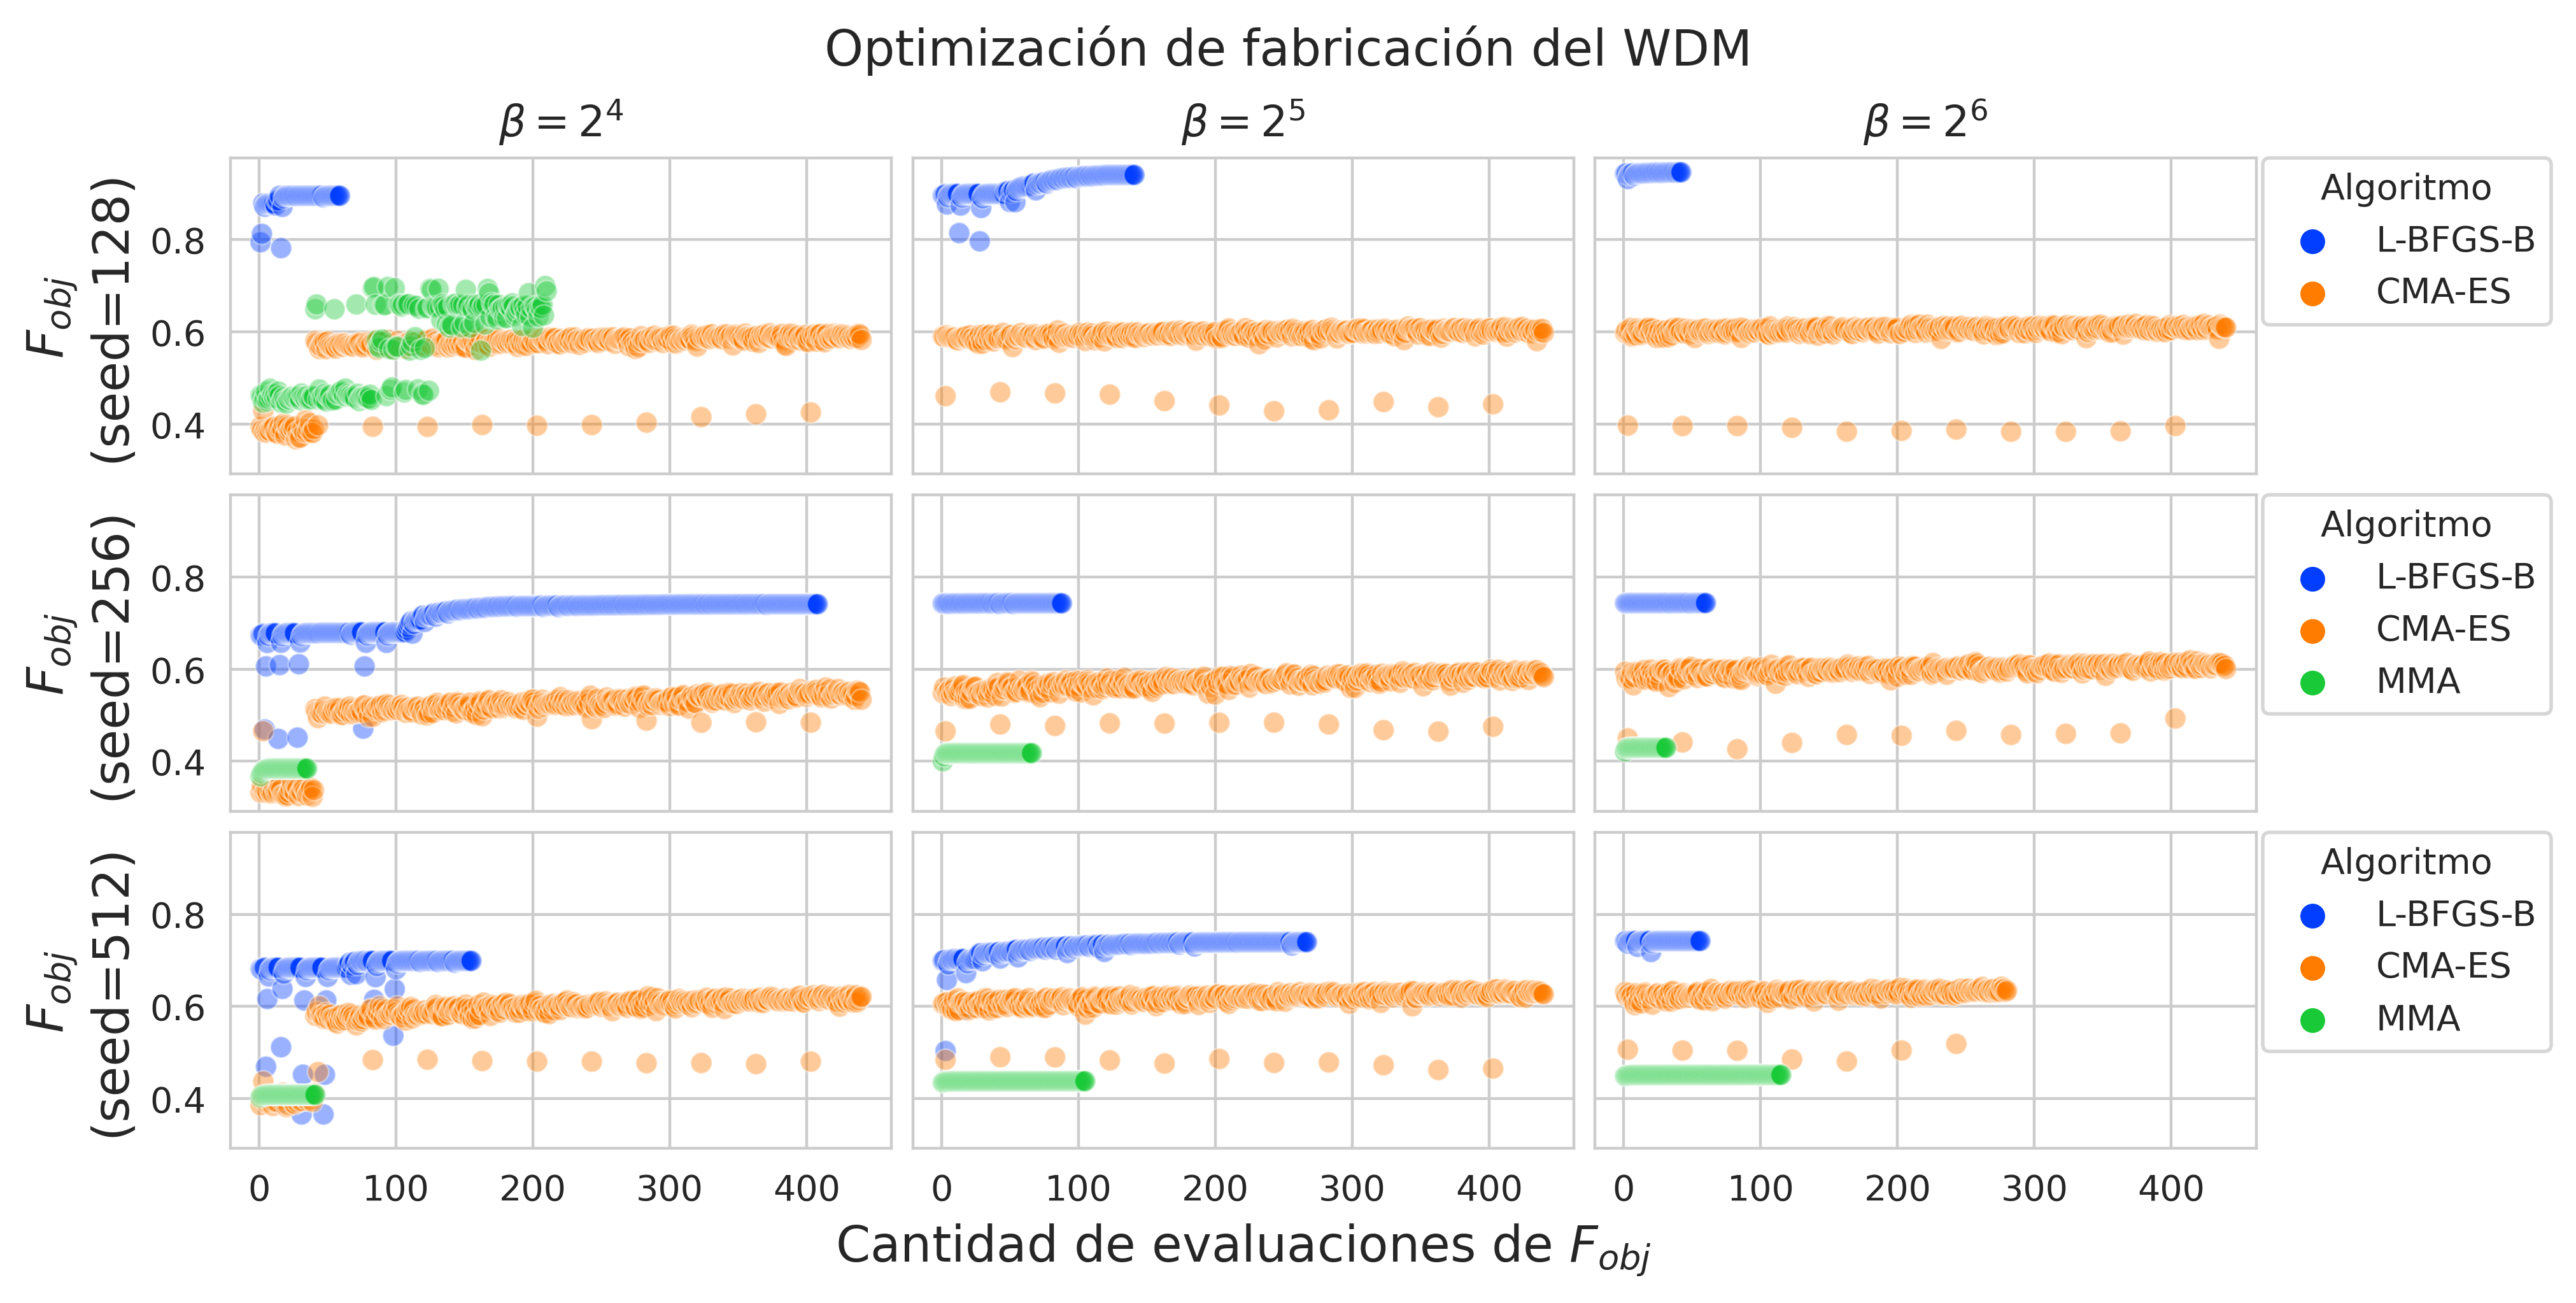
\includegraphics[scale=1.0]{image/results/wdm/wdm-opt-fab.png}
  \caption{Gráfico de valores de $F_{obj}$ obtenidos por los algoritmos en la optimización de fabricación del WDM}
  \label{fig:wdm-fab}
\end{figure}
\end{landscape}

\begin{figure}[ht]
  \centering

  % 1° row
  \subfigure[Diseño nominal.]
  {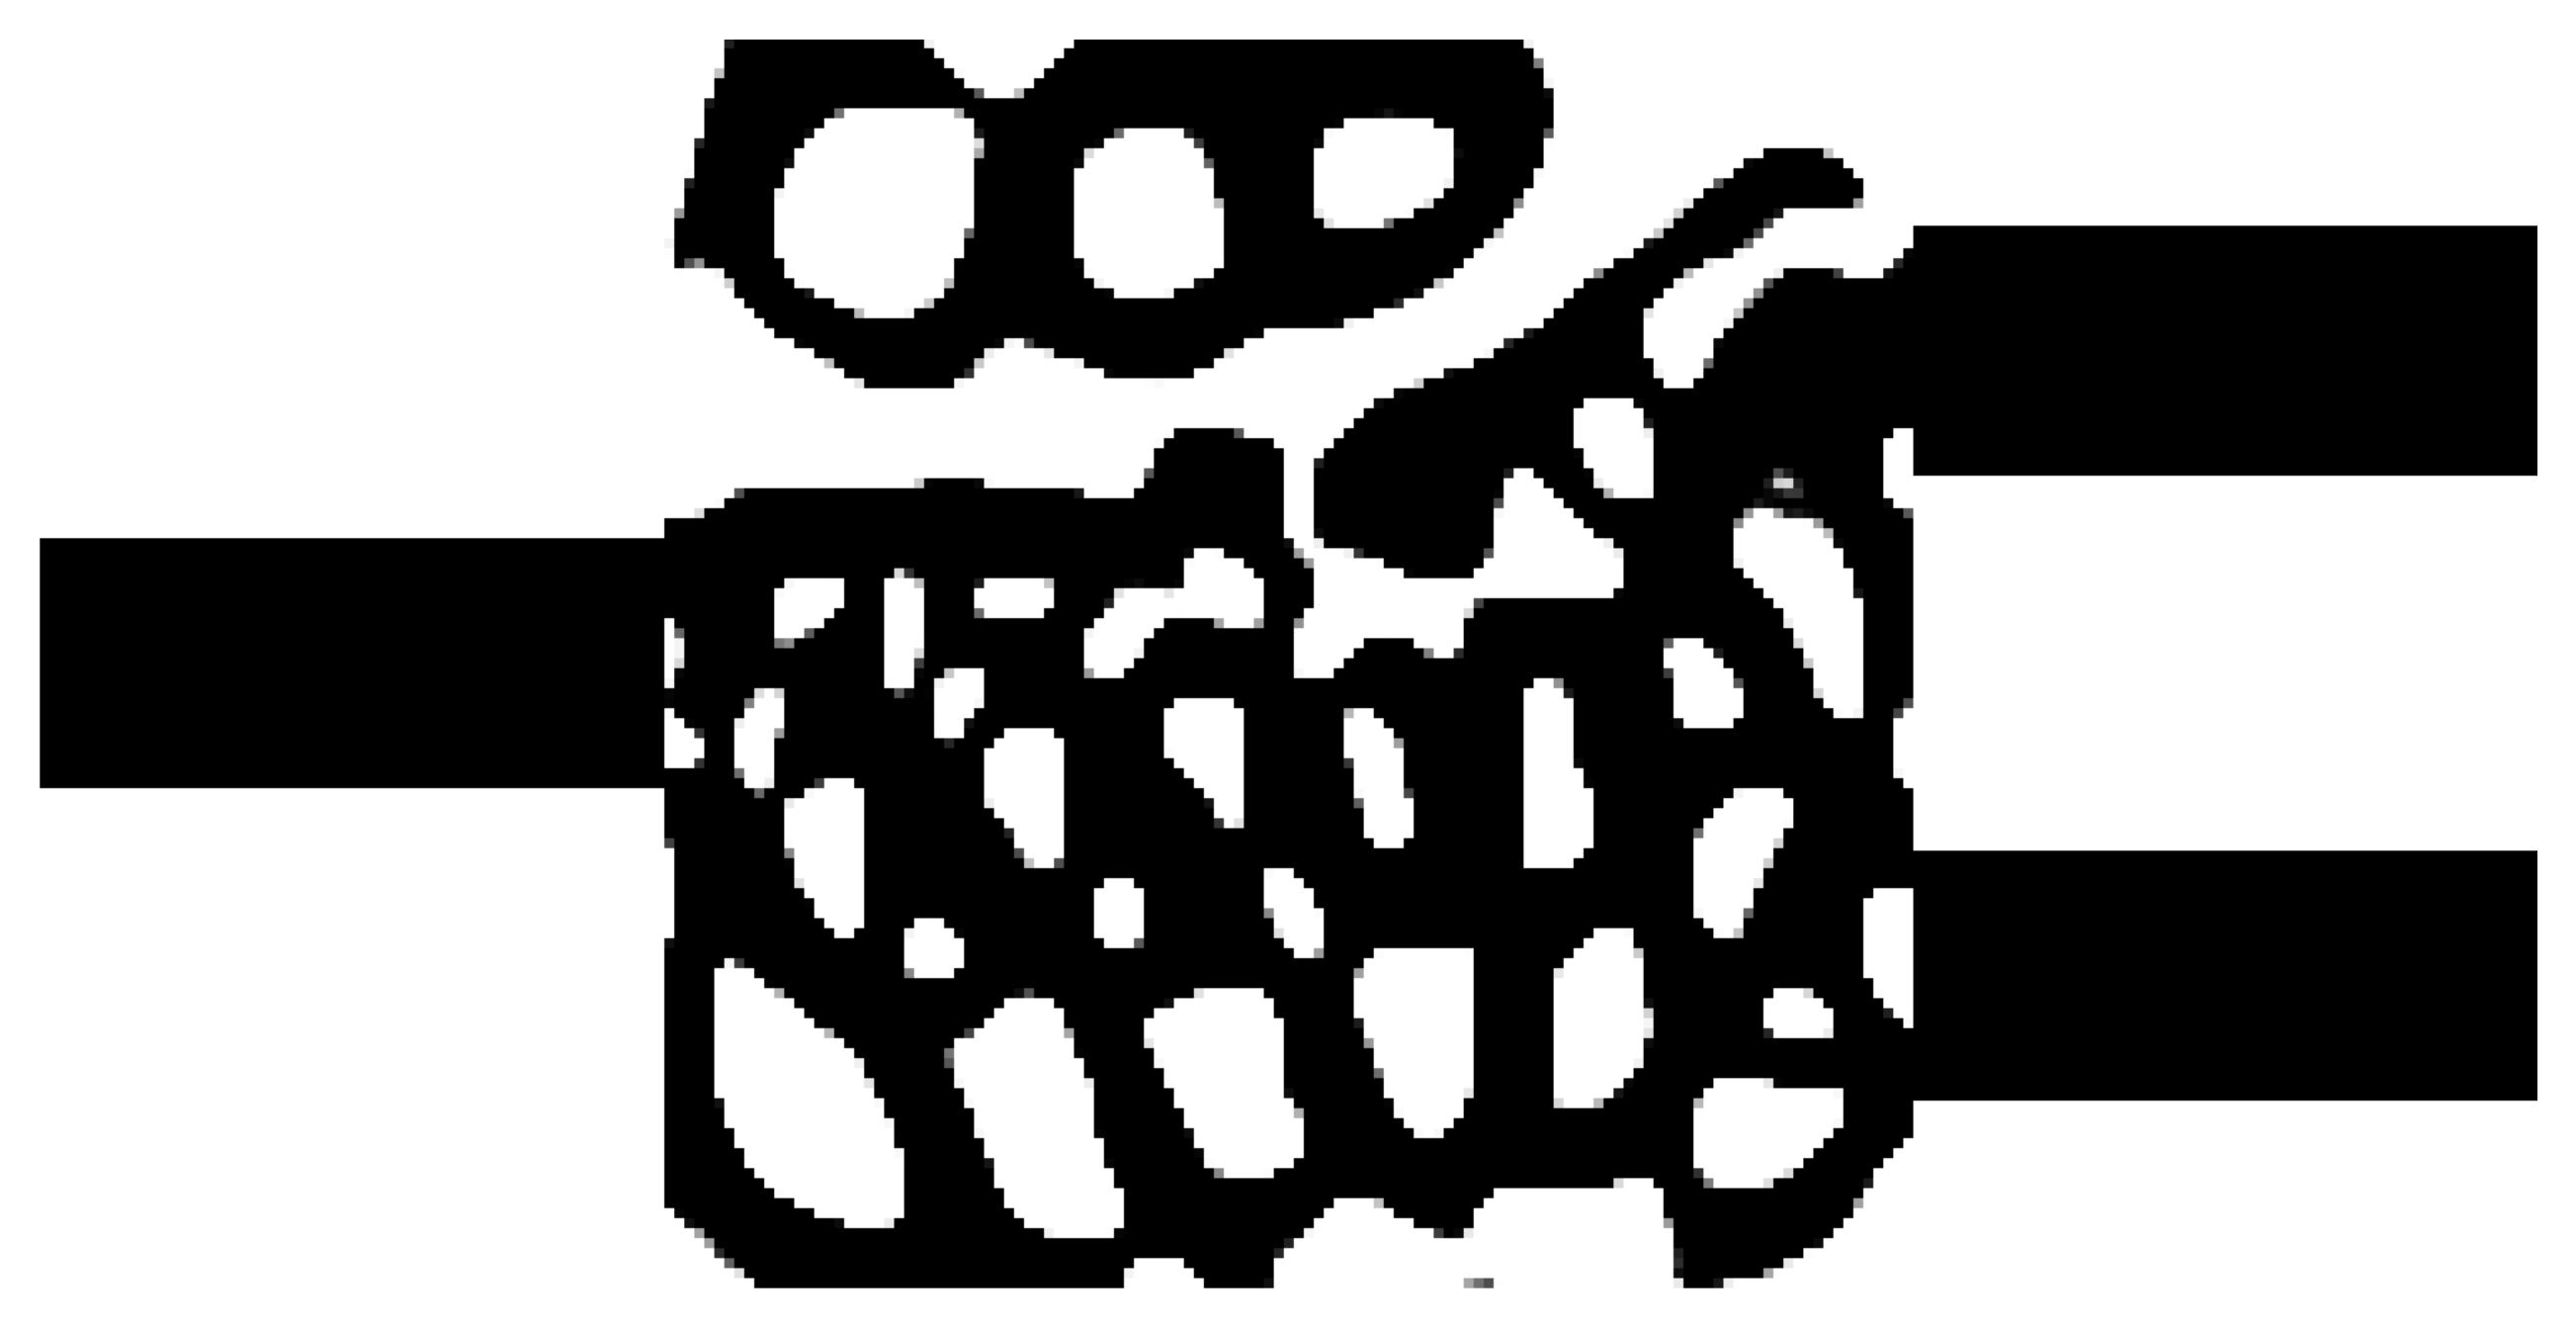
\includegraphics[width=0.48\textwidth]{image/results/wdm/best/eps.png}}
  \hfill
  \subfigure[Diseño nominal tras eliminar regiones no conexas.]
  {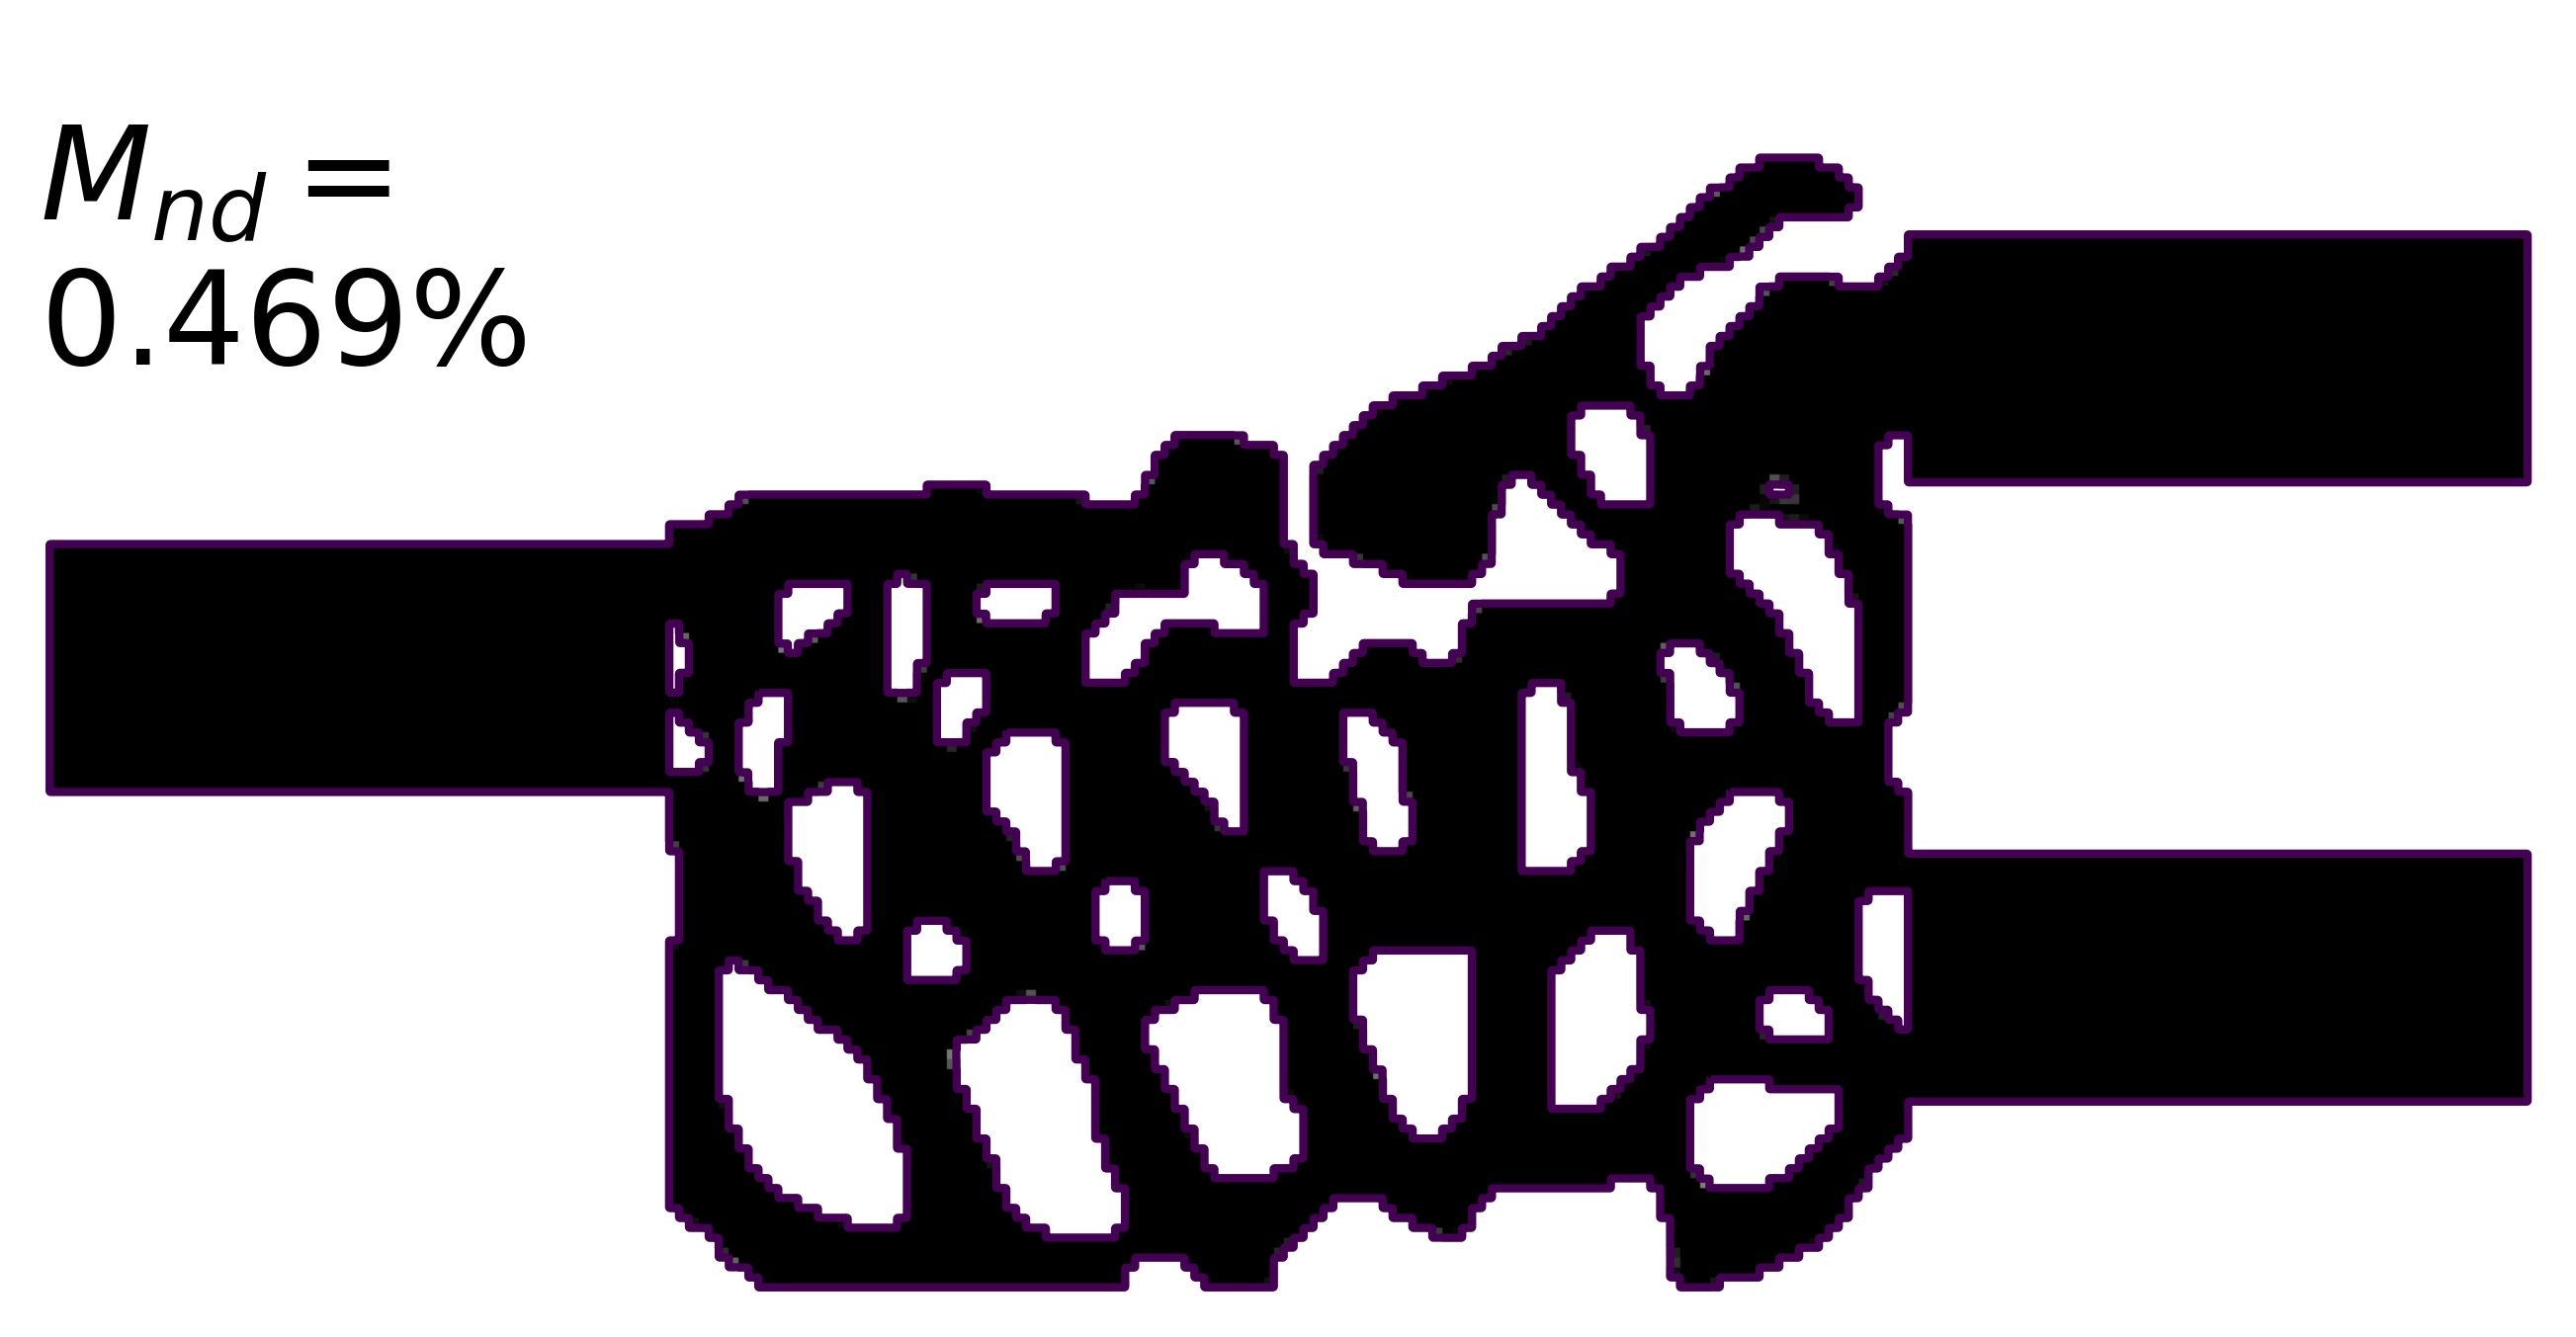
\includegraphics[width=0.48\textwidth]{image/results/wdm/best/eps_post.png}}

  % 2° row
  \subfigure[Campo $|\boldsymbol{E}|^2$ del diseño nominal.]
  {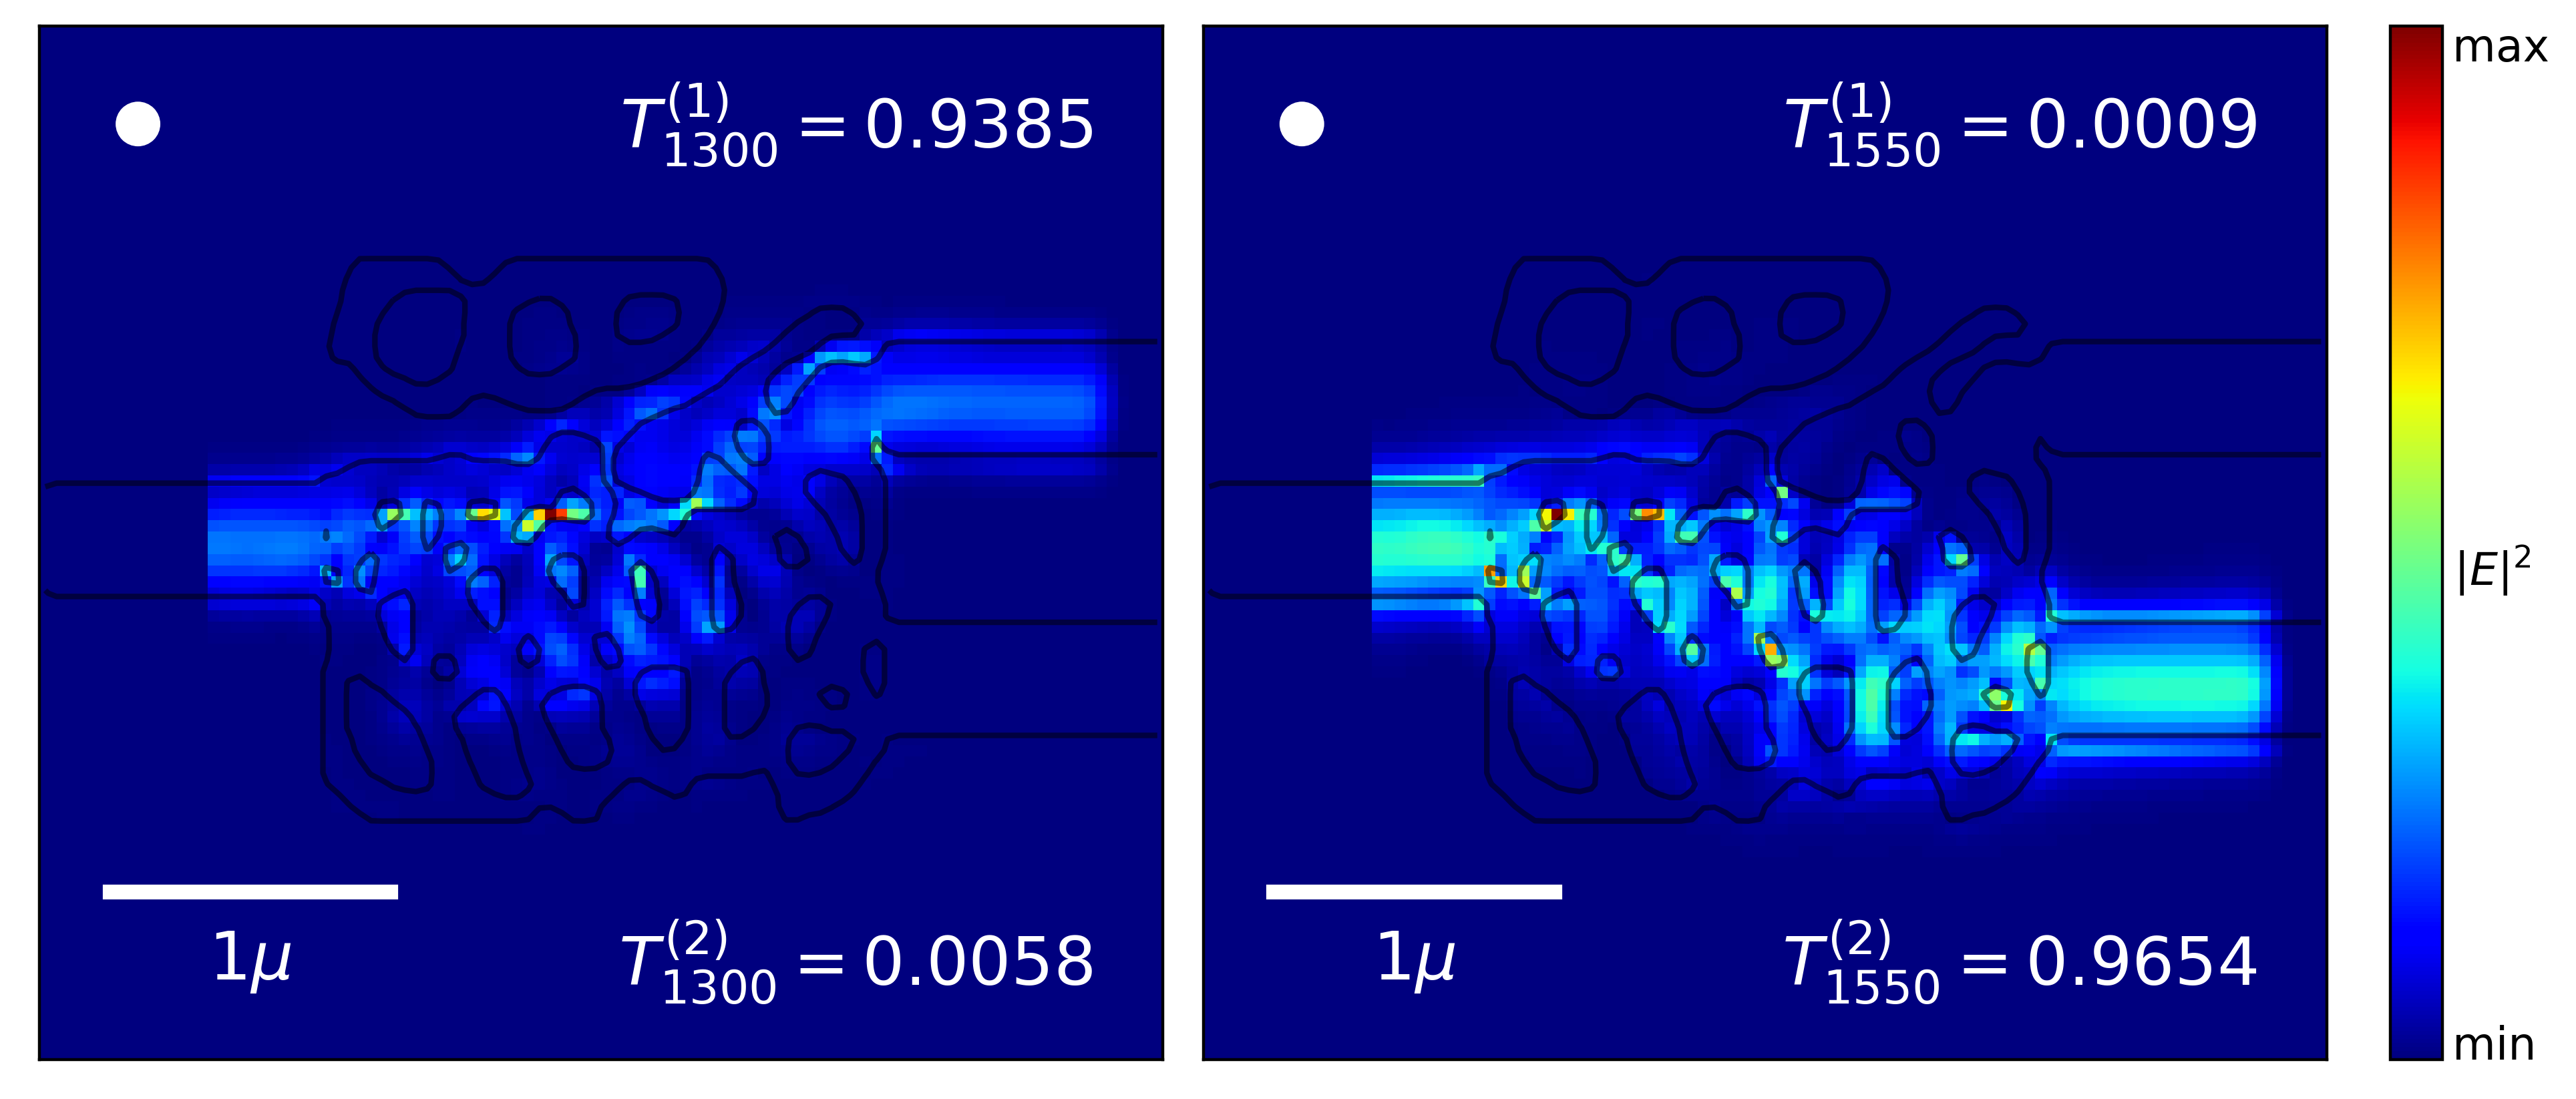
\includegraphics[width=0.48\textwidth]{image/results/wdm/best/field.png}}
  \hfill
  \subfigure[Campo $|\boldsymbol{E}|^2$ del diseño nominal tras eliminar regiones no conexas.]
  {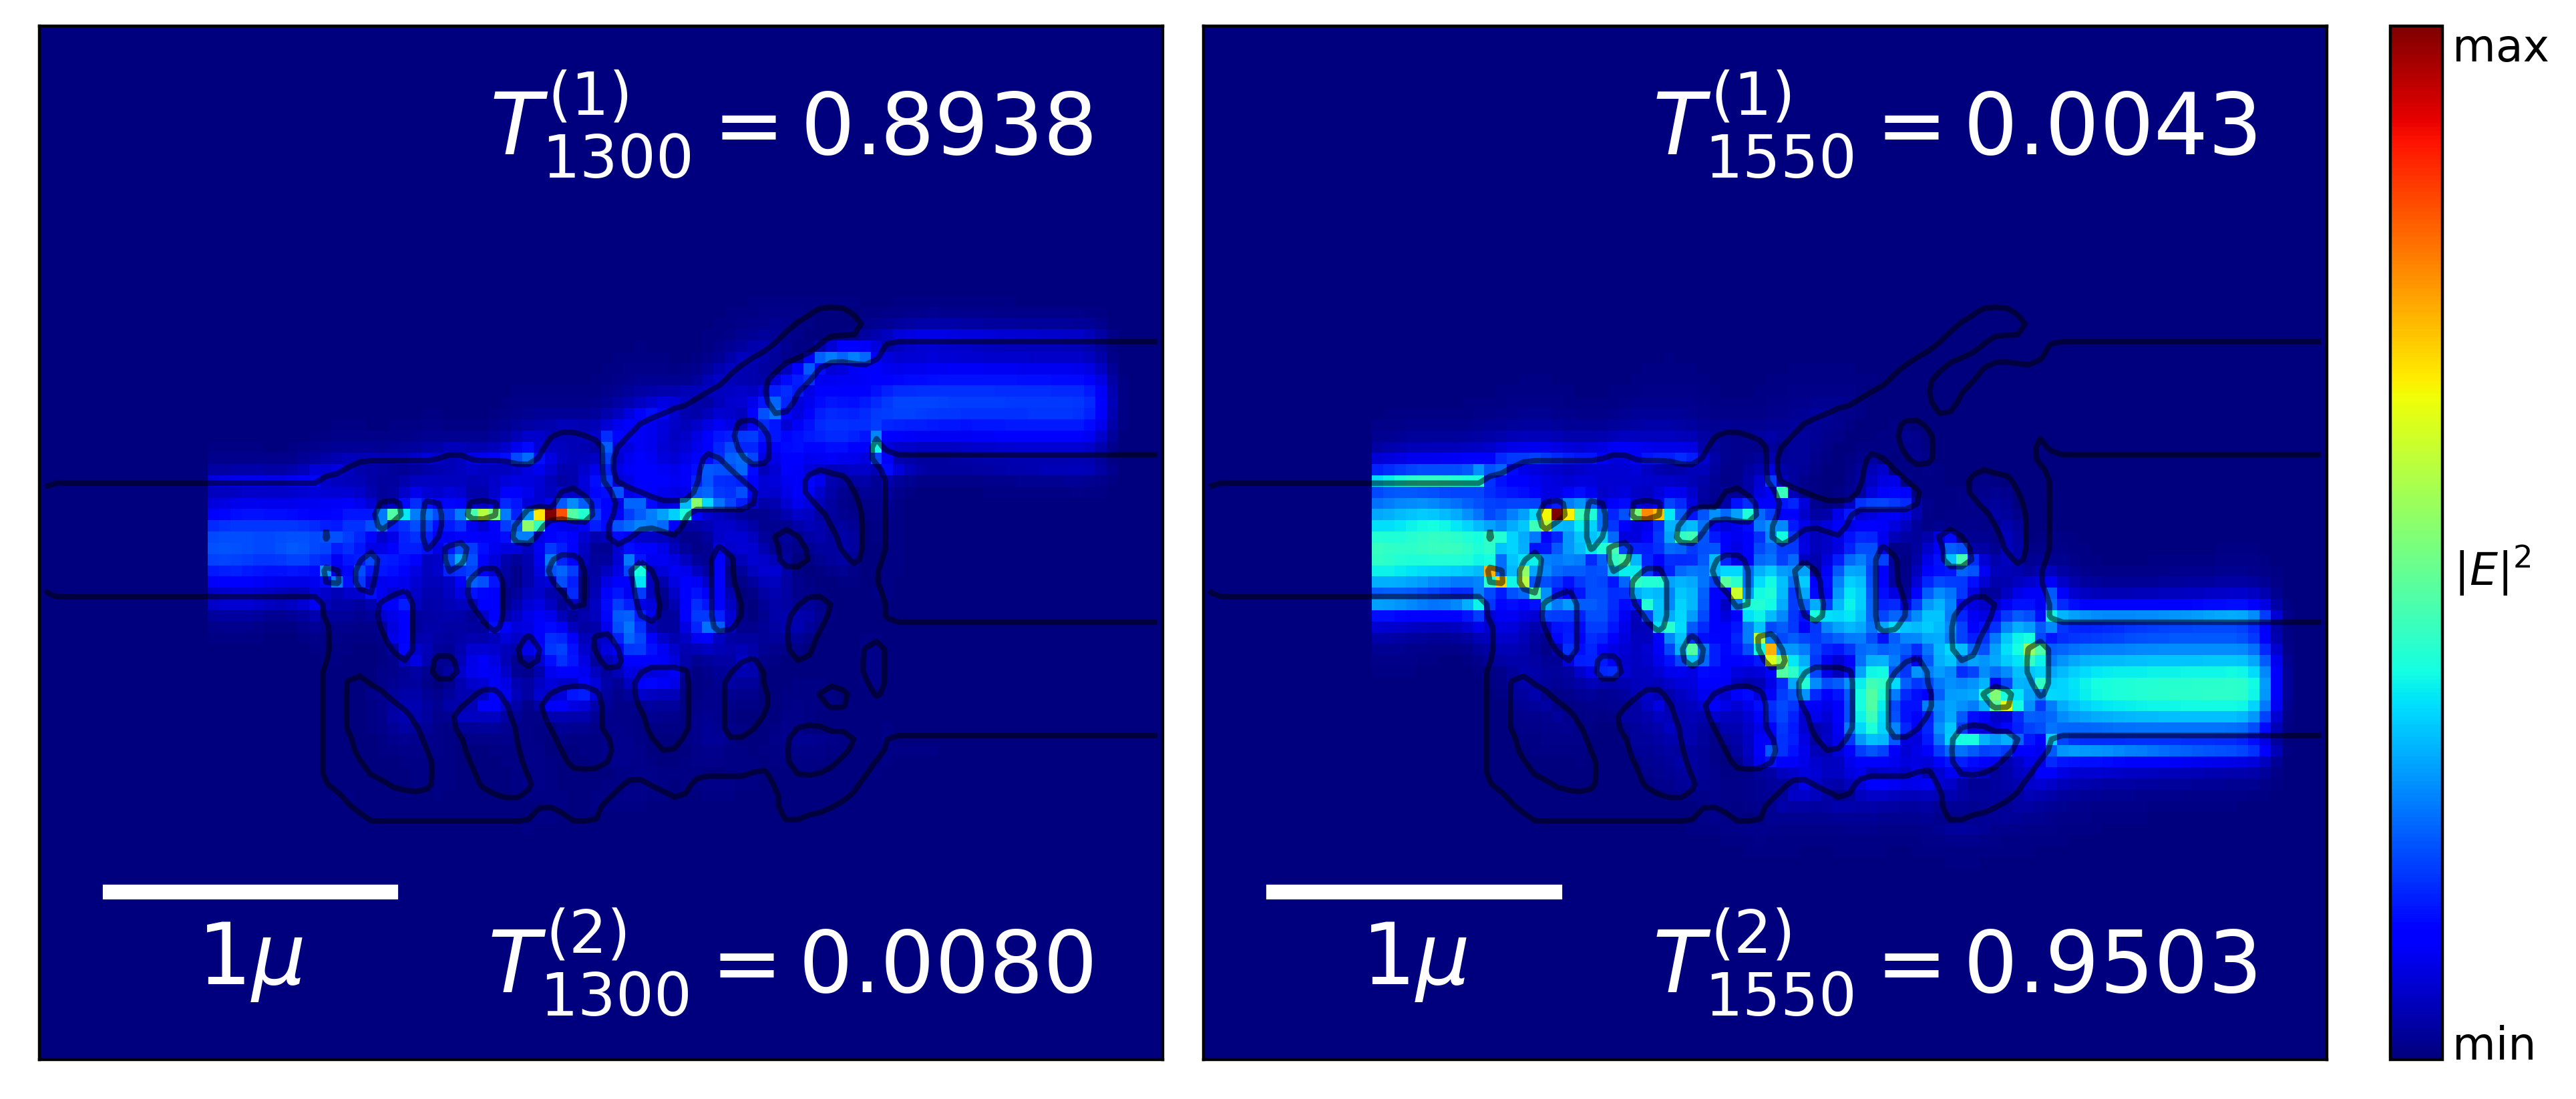
\includegraphics[width=0.48\textwidth]{image/results/wdm/best/field_post.png}}

  % 3° row
  \subfigure[Representación GDSII del diseño nominal.]
  {\includesvg[width=0.48\textwidth]{image/results/wdm/best/wdm.svg}}
  \hfill
  \subfigure[Representación GDSII del diseño nominal tras eliminar regiones no conexas.]
  {\includesvg[width=0.48\textwidth]{image/results/wdm/best/wdm_post.svg}}

  \caption{Posprocesamiento del diseño del WDM mejor optimizado.}
  \label{fig:bestwdm}

\end{figure}

\section{Diseño del WDM Mejor Optimizado}\label{sec:best-wdm}

De la sección anterior tenemos que el WDM mejor optimizado se consiguió
utilizando el algoritmo L-BFGS-B con un \emph{seed} (valor de semilla) de 128.

Al aplicar la \autoref{eq:grayscale} obtenemos que el porcentaje de región gris en el diseño
es de 1.233 \%, un valor menor a 2 \%, por lo cual podemos considerar que el diseño ha sido
adecuadamente binarizado. 
Por otro lado, si eliminamos las regiones no conectadas con la guía de entrada
tenemos un diseño con un porcentaje de gris de 0.469 \%.
Estos diseños lo podemos observar en la \autoref{fig:bestwdm},
el contorno morado alrededor de las geometrías de (a) y (b) representan los polígonos
usados para aproximar estas geometrías con el fin de obtener la descripción en el formato
GDSII, lo cual se puede observar en (e) y (f).
Adicionalmente, en la \autoref{fig:broadband-wdm} se muestra el comportamiento del diseño
en un rango de longitudes de onda de $1250nm$ a $1600 nm$, resultados obtenidos usando una ventana de $50nm$.
En este rango, considerando los errores de erosión y dilatación, 
para el diseño nominal la máxima diferencia de transmitancia 
es de 0.108 en la guía de onda superior y de 0.116 en la guía de onda inferior.
De manera similar, para el diseño nominal tras eliminar regiones no conexas,
la máxima diferencia de transmitancia
es de 0.114 en la guía de onda superior y de 0.098 en la guía de onda inferior.

\begin{figure}[ht]
  \centering
  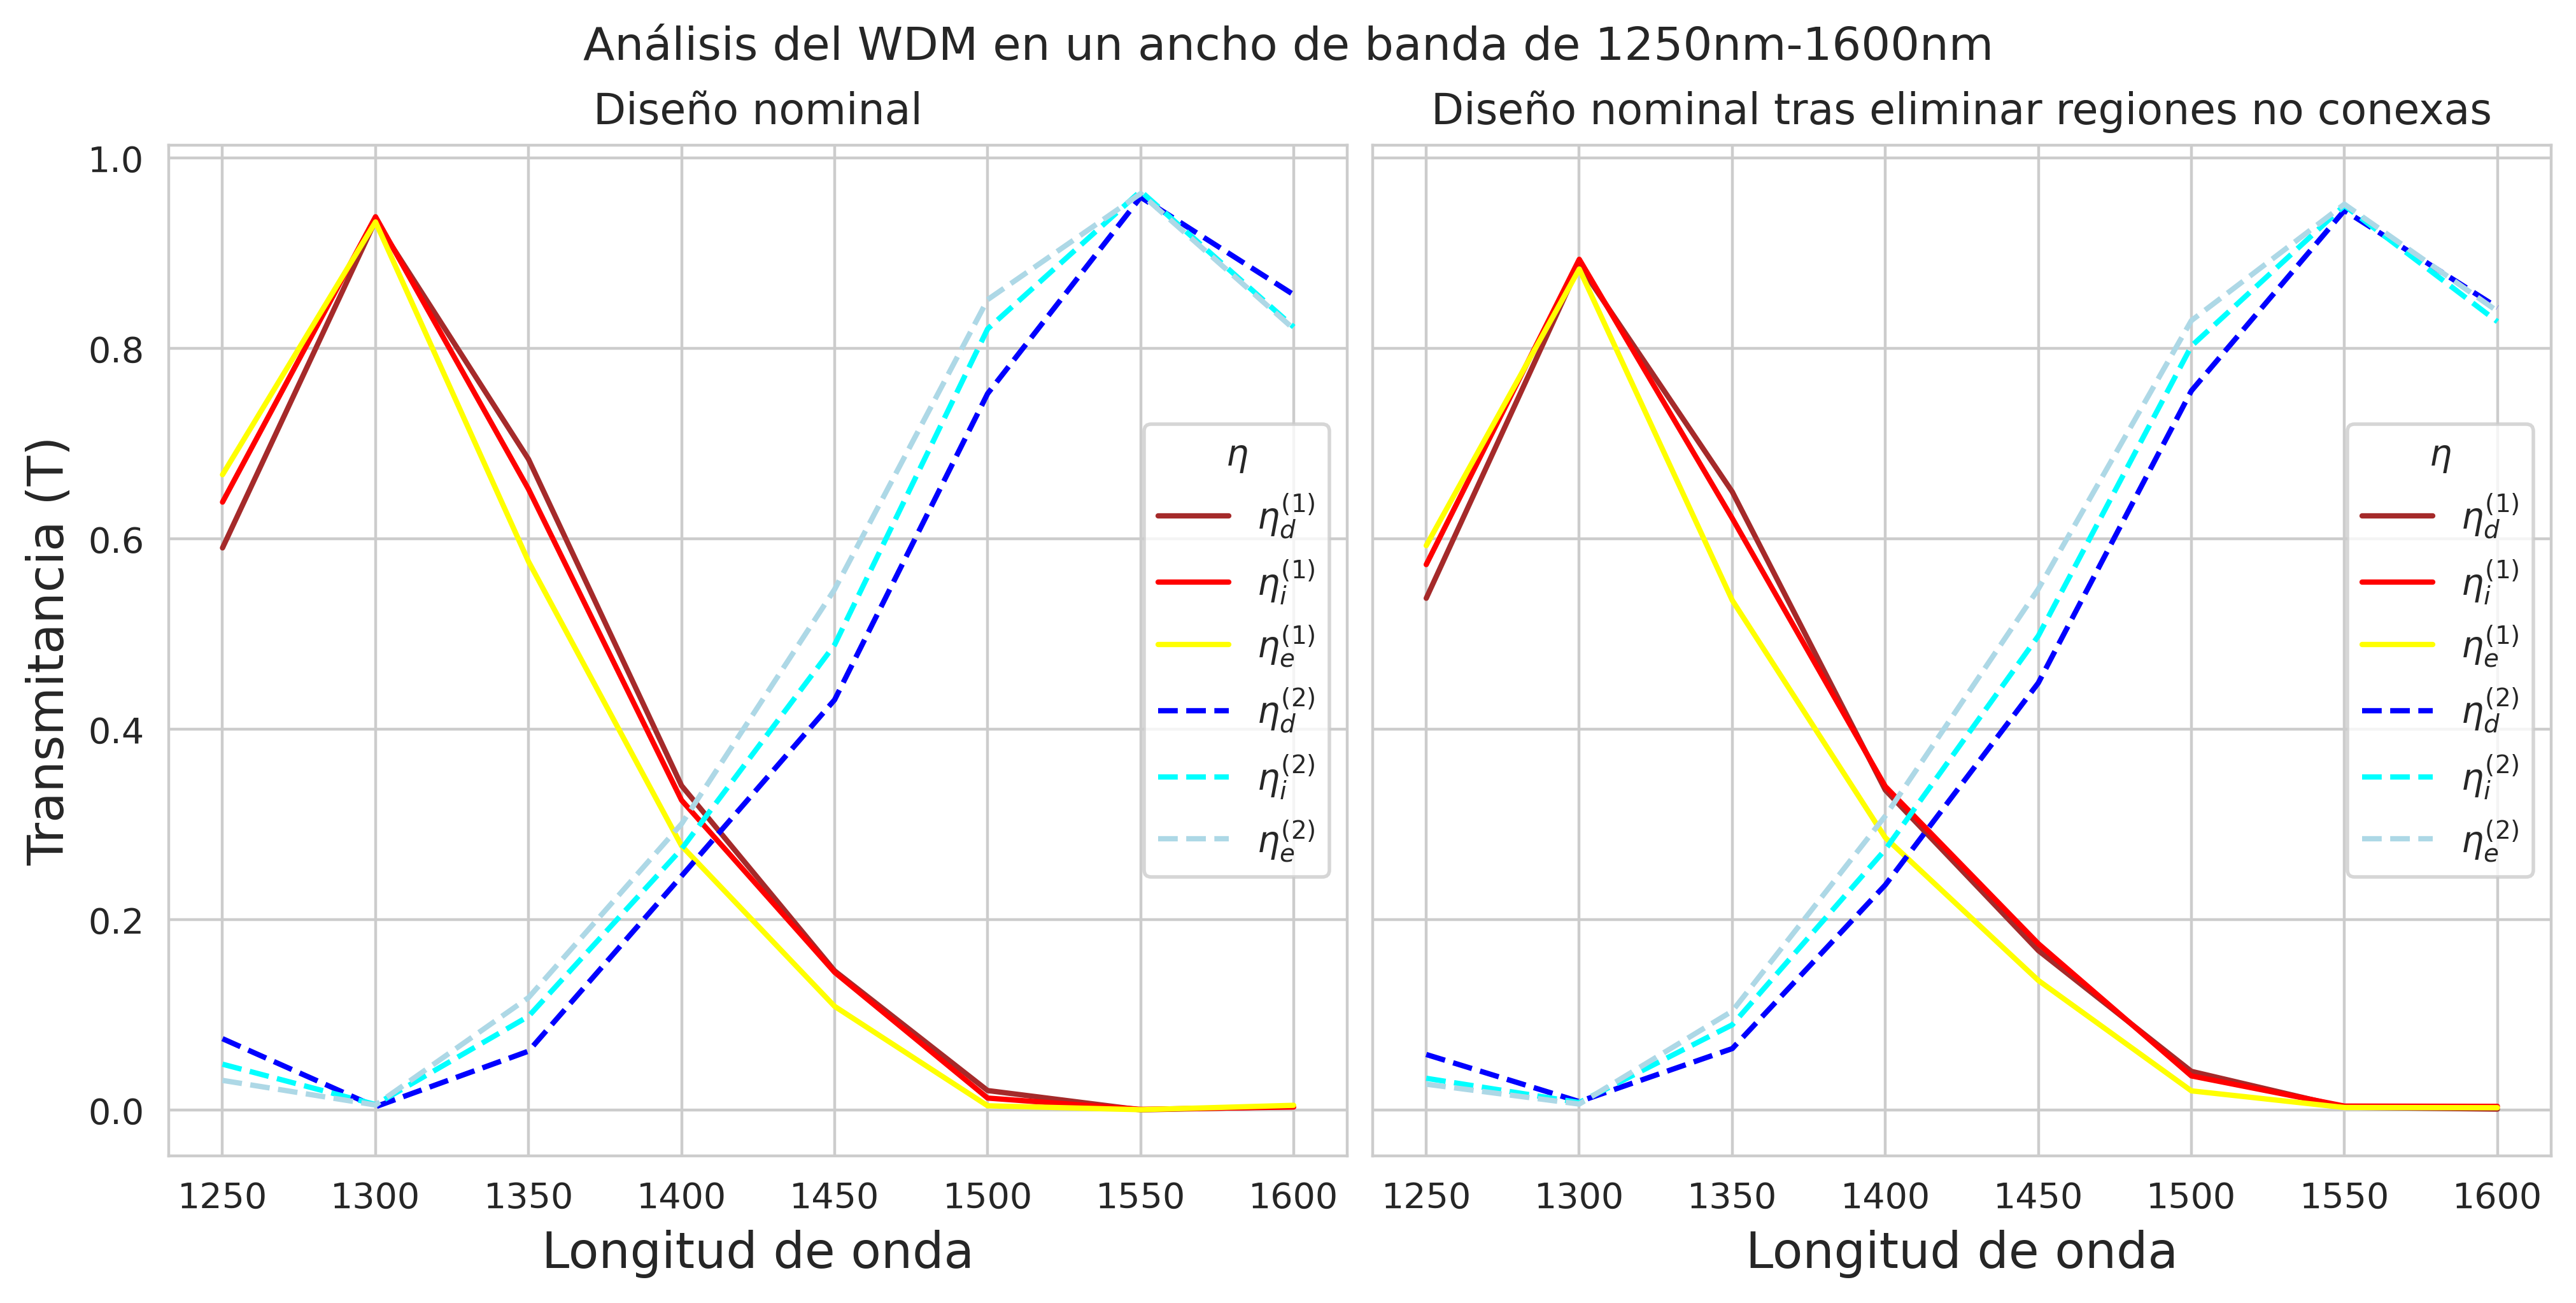
\includegraphics[width=\textwidth]{image/results/wdm/best/broadband-wdm.png}
  \caption{Análisis del WDM mejor optimizado en un rango de longitudes de onda ($1250 nm-1550 nm$)}
  \label{fig:broadband-wdm}
\end{figure}



\section{Discusión de Resultados del \emph{Bend}}

Para poder entender nuestros resultados buscamos una referencia del estado del arte
en la optimización de un \emph{bend}.
Sin embargo, en el mejor de nuestro conocimiento no hay publicaciones recientes que muestren
resultados explícitos en la optimización de un \emph{bend} de un área de diseño de $2 \mu m \times 2 \mu m$.
Pero, utilizando SPINS-B tenemos que el diseño intuitivo posee una transmitancia de $0.8399$ a $1550 nm$.

Luego, analizando la \autoref{fig:bend-cont}, \autoref{fig:bend-disc} y \autoref{fig:bend-fab}
pudimos comparar el desempeño y convergencia de los cinco algoritmos escogidos 
en la optimización del \emph{bend}.
En nuestro caso el desempeño viene dado por el valor de la FOM, a mayor FOM 
decimos que el algoritmo tuvo un mejor desempeño.
Particularmente, observamos que la optimización continua es la etapa que influye más
en los diseños finales encontrados. Esto tiene sentido pues las dos siguientes etapas
son principalmente para refinar los resultados de esta primera etapa en un diseño
fabricable.

Centrándonos en los resultados del MMA, lo primero que nos llamó
la atención de la optimización continua (\autoref{fig:bend-cont}) es el hecho que el algoritmo converge 
incluso antes de realizar 100 evaluaciones de $f_{obj}$. 
Al inicio pensamos que era un error de configuración,
pero incluso si forzábamos al algoritmo a realizar todas las evaluaciones permitidas, 
este se estancaba en diseños con transmitancias cercanas a 0.
Además, esta misma tendencia se repitió en la optimización discreta (\autoref{fig:bend-disc})
y la optimización de fabricación (\autoref{fig:bend-fab}).
Por último, en la \autoref{tab:opt-MMA-bend} observamos que los diseños 
ni siquiera lograron conectar las guías de onda.
En conclusión, si bien este algoritmo converge rápidamente, en términos de desempeño
es el peor algoritmo de los estudiados para el caso del \emph{bend}.
De hecho, tenemos que MMA fue el único algoritmo que no logró conectar las guías de onda y
que no logró obtener un diseño con mejor transmitancia que el diseño intuitivo.

Centrándonos en los resultados del G-CMA-ES, notamos que después del MMA este algoritmo
obtuvo los diseños con menor transmitancia en las tres etapa de optimización;
además, en promedio fue quien más se demoró en converger
(\autoref{fig:bend-cont}, \autoref{fig:bend-disc} y \autoref{fig:bend-fab}).
Seguidamente, en la \autoref{tab:opt-CMA-bend} pudimos apreciar que G-CMA-ES obtuvo geometrías 
con presencia de pequeñas zonas grises (en promedio, $M_{nd} = 5.459 \%$) y zonas puntiagudas.
En conclusión, tanto en términos de eficiencia como de convergencia este algoritmo no
mostró los mejores resultados.

Centrándonos en los resultados de los restantes algoritmos (L-BFGS-B, G-PSO y G-GA)
notamos que los tres lograron encontrar diseños con transmitancias mayores al $90 \%$
en todas las etapas de optimización. Sin embargo, L-BFGS-B mustró superioridad 
tanto en términos de eficiencia como de convergencia. Los otros dos algoritmos (G-PSO y G-GA)
obtuvieron valores del FOM ligeramente menores y necesitaron mayor tiempo de convergencia.
Adicionalmente, a partir de la \autoref{tab:opt-LBFGSB-bend}, \autoref{tab:opt-PSO-bend} y
\autoref{tab:opt-GA-bend} pudimos notar que en promedio solamente L-BFGS-B y G-PSO
generaron diseños adecuadamente binarizados ($M_{nd} < 2 \%$) y con poca presencia de regiones
puntiagudas.

En síntesis, se obversó que L-BFGS-B y G-PSO fueron las únicas opciones que lograron
producir dispositivos adecuadamente binarizados, con elevadas transmitancias y 
facilidad de fabricación.
A partir de las observaciones realizadas se elaboró una relación de orden entre los 
algoritmos de acuerdo a los criterios: 
(i) desempeño (mayor valor de $F_{obj})$, 
(ii) convergencia (más rápida, promedio de las tres etapas de optimización) y 
(iii) $M_{nd}$ promedio (menor porcentaje de gris).
Esto se puede encontrar en la \autoref{tab:order-bend}.

\begin{table}[ht]
    \centering
    \begin{tabular}{|c|c|c|}
    \hline 
    Desempeño &  Convergencia & $M_{nd} $\\
    \hline 
      L-BFGS-B (0.9895) & MMA (165)           &  L-BFGS-B (1.157 \%) \\
      G-PSO (0.9830)    & L-BFGS-B (566)    & G-PSO (1.519 \%) \\
      G-GA (0.9744)     & G-PSO (3094)    & G-GA (2.062 \%) \\
      G-CMA-ES (0.9155) & G-GA (3117)     & G-CMA-ES (5.459 \%) \\
      MMA (0.0383)      & G-CMA-ES (3320) & MMA (23.958 \%) \\
    \hline 
    \end{tabular}
    \caption{Relación de orden de los algoritmos en la optimización del \emph{bend} según
             los criterios de (i) desempeño, (ii) convergencia y (iii) $M_{nd}$.}
    \label{tab:order-bend}
\end{table}


Por último, sin contar al MMA, los algoritmos produjeron pequeñas ``islas''
(regiones no conexas entre las guía de entrada y la guía de salida).
En la \autoref{sec:best-bend} se utilizó el diseño mejor optimizado para experimentar
quitando estos elementos. 
Sorprendentemente, estos resultados siguieron teniendo una transmitancia
mayor a 90 \%.
Incluso si trabajamos en longitudes de onda en el rango de $1500nm-1600nm$
los resultados se mantienen similares aún cuando pueda ocurrir errores de erosión o dilatación.
De este modo, se comprobó que el diseño obtenido es eficiente y robusto no solo a errores
de fabricación, sino que también es flexible en la longitud de onda con la que puede trabajar.

\section{Discusión de Resultados del WDM}

Para poder entender nuestros resultados buscamos una referencia del estado del arte en la optimización
de un WDM. Así, encontramos que 
\cite{Piggott2015} optimizaron un WDM con una región de diseño de $2.8 \mu m \times 2.8 \mu m$
trabajando a $1300 nm$ y $1550 nm$. En su trabajo muestran los resultados en gráficas por lo cual
es dificil encontrar los valores exactos de transmitancia reportados. Sin embargo, en
\cite{Sigmund2016} se detalla que el diseño obtenido posee 
$T_{1310}^{(1)} = 0.8377$ y $T_{1550}^{(2)} = 0.8076$.
También existen trabajos como los de \cite{Christiansen2021} y \cite{Zhang2021} que optimizan
un WDM; pero, realizaron las simulaciones en 2D por lo cual la comparación no es justa.

Como se observa en la \autoref{sec:best-wdm}, el diseño del WDM mejor optimizado en este trabajo posee $T_{1300}^{(1)} = 0.9385$ y 
$T_{1550}^{(2)} = 0.9503$ y tras eliminar las regiones no conexas obtiene
$T_{1300}^{(1)} = 0.8938$ y $T_{1550}^{(2)} = 0.9503$. Además, al realizar el análisis
en un rango de longitudes de onda de $1250nm-1600nm$ obtuvimos un comportamiento similar
al logrado en \cite{Piggott2015}.
De este modo, aparentemente hemos obtenido un diseño que supera el estado del arte en
simulaciones 3D.
Sin embargo, es necesario fabricar estos diseños para corroborar los resultados de las simulaciones.

Por otro lado, centrándonos en los resultados del MMA, tenemos que al igual que sucedió con el \emph{bend},
el algoritmo no logró llegar a diseños que al menos conecten las guías de onda, 
ver \autoref{tab:opt-MMA-wdm}.
Primero, se consideró la posibilidad de haber algún error en el cálculo de la gradiente;
sin embargo, otros algoritmos si han logrado encontrar diseños funcionales tanto del
\emph{bend} como del WDM. Así, este escenario es poco probable.
Además, para la configuración del algoritmo se utilizó como guía un tutorial de MEEP \citep{Oskooi2010},
por lo que un error de configuración también parece sensato de descartarse.
Probablemente, el algoritmo simplemente requería de una cantidad mayor de iteraciones.

Respecto al desempeño de los demás algoritmos, notamos que se cumplía una tendencia similar
al caso del \emph{bend} respecto al desempeño de los algoritmos: MMA tuvo el peor
desempeño con dispositivos con geometrías sin forma definida y no funcionales
(\autoref{tab:opt-MMA-wdm}), G-CMA-ES obtuvo los siguientes mejores resultados,
pero incluía un gran porcentaje de región gris en sus diseños y regiones puntiagudas.
Finalmente, omitiendo el valor de semilla de 128, L-BFGS-B, G-CMA-ES y G-PSO obtuvieron
desempeños similares.
Sin embargo, en promedio L-BFGS-B fue el único algoritmo que encontró geometrías
adecuadamente binarizadas. De esta manera, se intuye que era necesario más iteraciones
en la etapa de optimización para asegurar un menor porcentaje de gris.

Particularmente, si bien todos los algoritmos (a excepción del MMA) lograron conectar
una guía de salida con la guía de entrada, solo una instancia del L-BFGS-B y del G-PSO
consiguieron diseños que conectaron ambas guías de salida de manera funcional,
las demás optimizaciones prefirieron mantener la guía de salida superior disconexa
y buscar alcanzar una trasmitancia cercana a 1 en el brazo inferior a $1550 nm$.
Así, parece sensato concluir que la definición de nuestra función objetivo aún carece de un
término que incentive en mayor medida que ambas guías de salida queden conectadas.

En síntesis, se observó que L-BFGS-B fue la única opcion que logró
producir un diseño adecuadamente binarizado, con elevadas transmitancias y 
facilidad de fabricación.
A partir de las observaciones realizadas se elaboró una relación de orden entre los 
algoritmos de acuerdo a los criterios: 
(i) desempeño (mayor valor de $F_{obj})$, 
(ii) convergencia (más rápida, promedio de las tres etapas de optimización) y 
(iii) $M_{nd}$ promedio (menor porcentaje de gris).
Esto se puede encontrar en la \autoref{tab:order-wdm}.

\begin{table}[ht]
    \centering
    \begin{tabular}{|c|c|c|}
    \hline 
    Desempeño &  Convergencia & $M_{nd} $\\
    \hline 
      L-BFGS-B (0.9465) & MMA (168)      &  L-BFGS-B (1.237 \%) \\
      G-PSO (0.8005)    & L-BFGS-B (946) & G-PSO (2.224 \%) \\
      G-GA (0.7176)     & G-GA (2137)     & G-GA (4.300 \%) \\
      G-CMA-ES (0.6427) & G-PSO (3103)    & G-CMA-ES (7.977 \%) \\
      MMA (0.4594)      & G-CMA-ES (3320) & MMA (23.898 \%) \\
    \hline 
    \end{tabular}
    \caption{Relación de orden de los algoritmos en la optimización del WDM según
             los criterios de (i) desempeño, (ii) convergencia y (iii) $M_{nd}$.}
    \label{tab:order-wdm}
\end{table}

En este capítulo hemos desarrollado la propuesta presentada en el \autoref{chapter:methodology}.
Primero, se realizó una descripción de los resultados de la optimización del \emph{bend} y 
se analizó al mejor diseño obtenido. 
Luego, se practicó la misma estrategia sobre los resultados del WDM.
Finalmente, hemos realizado una discusión crítica sobre estos resultados.
Así, como hemos podidos observar, hemos conseguido diseños eficientes y robustos tanto para un \emph{bend}
como para un WDM siguiendo la estrategia de optimización planteada.
